\NeedsTeXFormat{LaTeX2e}
\documentclass[a4paper,11pt]{article}
\usepackage[utf8]{inputenc}

\usepackage[affil-it]{authblk}
\usepackage{natbib}

\usepackage{setspace}

\usepackage{booktabs}
\usepackage{amsmath}
\usepackage{amssymb}
\usepackage{epsfig}

\usepackage{marvosym}

\usepackage{graphicx}
\usepackage{caption}
\usepackage{subcaption}
\usepackage{multicol}
\usepackage{etoolbox}

\usepackage{todonotes}

\usepackage{tikz}

%\usepackage{hyperref}
\usepackage[nameinlink]{cleveref}

\setlength{\textheight}{9in}
\setlength{\textwidth}{6in}
\setlength{\oddsidemargin}{.25in}
\setlength{\topmargin}{-.5in} 

\setcitestyle{authoryear, open={(},close={)}}
%\patchcmd{\thebibliography}{\section*{\refname}}
%    {\begin{multicols}{2}[\section*{\refname}\singlespace\footnotesize]}{}{}
%\patchcmd{\endthebibliography}{\endlist}{\endlist\end{multicols}}{}{}

\hyphenation{itself}

\title{{\small 02935 Introduction to applied statistics and R for PhD students: }\\[1em]Statistical report: Weather and travel demand}

\author{Niklas Christoffer Petersen}
\affil{Transport Modelling, Department of Management Engineering \\ Technical University of Denmark, 2800 Kongens Lyngby, Denmark}

%\affil{Trafikselskabet Movia \\ Technical University of Denmark, 2800 Kongens Lyngby, Denmark}

\begin{document}
\singlespace
\maketitle
\thispagestyle{empty}
\clearpage

\onehalfspacing
\pagenumbering{arabic}
\tableofcontents
\clearpage

\section{Background}\label{ch:background}

Observing and predicting the demand for bus travel is of major impact for designing and operating an efficient public transport system in any urban area. It is a common understanding, that there are several external factors that impact the travel demand. Examples include weather, events, etc. It is however uncertain how much each factor really contributes to fluctuation in travel demand. 

\subsection{Related work}\label{ch:relatedWork}
The impact of weather conditions on transport is a well-studied area within the scientific field of transport modeling.
TODO

For weather conditions, only sunny days and rainy days are considered: \citet{Yo2010}

\clearpage

\section{Data description}\label{ch:desc}
As established earlier, the goal of this project is to shed light upon the impact of specifically weather as an external factor for bus travel demand. For this, both historical weather data, and measures of historical travel demand should be analyzed.

\subsection{Travel demand data}\label{ch:desc_traveldemand}

Travel demand data was obtained and prepared as described in \Cref{appx:travel_demand_data_prep}. The preprocessed travel demand data is a quite simple time series containing number of passenger boardings for each date, time in terms of the hour of the day, and date of week. \Cref{tab:travel_demand_data_attr} shows the attributes in the travel demand date set, and \Cref{tab:travel_demand_data_example} shows an example of the data set.

\begin{table}[!ht]
    \center
    \begin{tabular}{p{1in}p{4in}}        
        Attribute & Description \\
        \hline 
        \hline         
        Date & The date of the observation (2016-10-01 - 2017-03-31). \\
        \hline 
        Hour & The hour of the observation (0--23, e.g.\ hour = 0 means between 00:00 and 01:00). \\
        \hline 
        Date of week & The day of the week of the observation (Mon - Sat), with statutory holidays encoded as Saturdays. \\
        \hline 
        Check in count & Number of passenger boardings using the smart-card ticketing system. \\
    \end{tabular}
    \caption{Attributes in the travel demand data set.}
    \label{tab:travel_demand_data_attr}
\end{table}

\begin{table}[!ht]
    \center
    %\includegraphics{../plots/travelcard_hist.pdf}
    \begin{tabular}{lllr}
 Date & Hour & Date of week & Check in count \\ 
  \hline
\hline
2016-10-01 & 0 & Sat & 280 \\ 
   \hline
2016-10-01 & 1 & Sat & 251 \\ 
   \hline
2016-10-01 & 2 & Sat & 153 \\ 
   \hline
2016-10-01 & 3 & Sat & 180 \\ 
   \hline
2016-10-01 & 4 & Sat & 151 \\ 
   \hline
2016-10-01 & 5 & Sat & 105 \\ 
   \hline
2016-10-01 & 6 & Sat & 130 \\ 
   \hline
2016-10-01 & 7 & Sat & 116 \\ 
   \hline
2016-10-01 & 8 & Sat & 228 \\ 
   \hline
2016-10-01 & 9 & Sat & 517 \\ 
  \end{tabular}

    \caption{Example of the travel demand data set.}
    \label{tab:travel_demand_data_example}
\end{table}


\Cref{fig:travelcard_boxplot} shows the boxplot of passenger boardings over the different days of week, where the notches gives a roughly 95\% confidence interval for comparing medians cf.~\citet{Boxplots}. The plot suggests that travel demand of Monday--Thursday could follow quite similar distributions, while Friday, Saturday and Sunday seems to each have a distinct travel demand distribution from the rest of the week.

\clearpage
\begin{figure}[!ht]
    \center
    %\includegraphics{../plots/travelcard_hist.pdf}
    % !TEX encoding = UTF-8 Unicode
\begin{tikzpicture}[x=1pt,y=1pt]
\definecolor{fillColor}{RGB}{255,255,255}
\path[use as bounding box,fill=fillColor,fill opacity=0.00] (0,0) rectangle (433.62,216.81);
\begin{scope}
\path[clip] (  0.00,  0.00) rectangle (433.62,216.81);
\definecolor{drawColor}{RGB}{255,255,255}
\definecolor{fillColor}{RGB}{255,255,255}

\path[draw=drawColor,line width= 0.6pt,line join=round,line cap=round,fill=fillColor] (  0.00,  0.00) rectangle (433.62,216.81);
\end{scope}
\begin{scope}
\path[clip] ( 47.21, 34.62) rectangle (427.62,210.81);
\definecolor{fillColor}{RGB}{255,255,255}

\path[fill=fillColor] ( 47.21, 34.62) rectangle (427.62,210.81);
\definecolor{drawColor}{gray}{0.98}

\path[draw=drawColor,line width= 0.6pt,line join=round] ( 47.21, 66.84) --
	(427.62, 66.84);

\path[draw=drawColor,line width= 0.6pt,line join=round] ( 47.21,116.24) --
	(427.62,116.24);

\path[draw=drawColor,line width= 0.6pt,line join=round] ( 47.21,165.65) --
	(427.62,165.65);
\definecolor{drawColor}{gray}{0.90}

\path[draw=drawColor,line width= 0.2pt,line join=round] ( 47.21, 42.14) --
	(427.62, 42.14);

\path[draw=drawColor,line width= 0.2pt,line join=round] ( 47.21, 91.54) --
	(427.62, 91.54);

\path[draw=drawColor,line width= 0.2pt,line join=round] ( 47.21,140.95) --
	(427.62,140.95);

\path[draw=drawColor,line width= 0.2pt,line join=round] ( 47.21,190.35) --
	(427.62,190.35);

\path[draw=drawColor,line width= 0.2pt,line join=round] ( 78.91, 34.62) --
	( 78.91,210.81);

\path[draw=drawColor,line width= 0.2pt,line join=round] (131.74, 34.62) --
	(131.74,210.81);

\path[draw=drawColor,line width= 0.2pt,line join=round] (184.58, 34.62) --
	(184.58,210.81);

\path[draw=drawColor,line width= 0.2pt,line join=round] (237.41, 34.62) --
	(237.41,210.81);

\path[draw=drawColor,line width= 0.2pt,line join=round] (290.25, 34.62) --
	(290.25,210.81);

\path[draw=drawColor,line width= 0.2pt,line join=round] (343.08, 34.62) --
	(343.08,210.81);

\path[draw=drawColor,line width= 0.2pt,line join=round] (395.92, 34.62) --
	(395.92,210.81);
\definecolor{drawColor}{RGB}{248,118,109}

\path[draw=drawColor,line width= 0.6pt,line join=round] ( 78.91,125.24) -- ( 78.91,190.85);

\path[draw=drawColor,line width= 0.6pt,line join=round] ( 78.91, 55.72) -- ( 78.91, 42.93);

\path[draw=drawColor,line width= 0.6pt,line join=round,line cap=round,fill=fillColor] ( 59.10,125.24) --
	( 59.10,100.72) --
	( 69.00, 96.24) --
	( 59.10, 91.75) --
	( 59.10, 55.72) --
	( 98.72, 55.72) --
	( 98.72, 91.75) --
	( 88.81, 96.24) --
	( 98.72,100.72) --
	( 98.72,125.24) --
	( 59.10,125.24) --
	cycle;

\path[draw=drawColor,line width= 1.1pt,line join=round] ( 69.00, 96.24) -- ( 88.81, 96.24);
\definecolor{drawColor}{RGB}{196,154,0}

\path[draw=drawColor,line width= 0.6pt,line join=round] (131.74,125.83) -- (131.74,181.76);

\path[draw=drawColor,line width= 0.6pt,line join=round] (131.74, 56.64) -- (131.74, 42.63);

\path[draw=drawColor,line width= 0.6pt,line join=round,line cap=round,fill=fillColor] (111.93,125.83) --
	(111.93,103.71) --
	(121.84, 99.25) --
	(111.93, 94.79) --
	(111.93, 56.64) --
	(151.56, 56.64) --
	(151.56, 94.79) --
	(141.65, 99.25) --
	(151.56,103.71) --
	(151.56,125.83) --
	(111.93,125.83) --
	cycle;

\path[draw=drawColor,line width= 1.1pt,line join=round] (121.84, 99.25) -- (141.65, 99.25);
\definecolor{drawColor}{RGB}{83,180,0}

\path[draw=drawColor,line width= 0.6pt,line join=round] (184.58,128.10) -- (184.58,193.51);

\path[draw=drawColor,line width= 0.6pt,line join=round] (184.58, 58.24) -- (184.58, 42.93);

\path[draw=drawColor,line width= 0.6pt,line join=round,line cap=round,fill=fillColor] (164.77,128.10) --
	(164.77,104.94) --
	(174.67,100.44) --
	(164.77, 95.93) --
	(164.77, 58.24) --
	(204.39, 58.24) --
	(204.39, 95.93) --
	(194.49,100.44) --
	(204.39,104.94) --
	(204.39,128.10) --
	(164.77,128.10) --
	cycle;

\path[draw=drawColor,line width= 1.1pt,line join=round] (174.67,100.44) -- (194.49,100.44);
\definecolor{drawColor}{RGB}{0,192,148}

\path[draw=drawColor,line width= 0.6pt,line join=round] (237.41,129.88) -- (237.41,202.80);

\path[draw=drawColor,line width= 0.6pt,line join=round] (237.41, 59.55) -- (237.41, 43.03);

\path[draw=drawColor,line width= 0.6pt,line join=round,line cap=round,fill=fillColor] (217.60,129.88) --
	(217.60,107.34) --
	(227.51,102.81) --
	(217.60, 98.27) --
	(217.60, 59.55) --
	(257.23, 59.55) --
	(257.23, 98.27) --
	(247.32,102.81) --
	(257.23,107.34) --
	(257.23,129.88) --
	(217.60,129.88) --
	cycle;

\path[draw=drawColor,line width= 1.1pt,line join=round] (227.51,102.81) -- (247.32,102.81);
\definecolor{drawColor}{RGB}{0,182,235}

\path[draw=drawColor,line width= 0.6pt,line join=round] (290.25,139.96) -- (290.25,199.94);

\path[draw=drawColor,line width= 0.6pt,line join=round] (290.25, 69.85) -- (290.25, 44.02);

\path[draw=drawColor,line width= 0.6pt,line join=round,line cap=round,fill=fillColor] (270.44,139.96) --
	(270.44,115.67) --
	(280.34,111.06) --
	(270.44,106.44) --
	(270.44, 69.85) --
	(310.06, 69.85) --
	(310.06,106.44) --
	(300.16,111.06) --
	(310.06,115.67) --
	(310.06,139.96) --
	(270.44,139.96) --
	cycle;

\path[draw=drawColor,line width= 1.1pt,line join=round] (280.34,111.06) -- (300.16,111.06);
\definecolor{drawColor}{RGB}{165,138,255}

\path[draw=drawColor,line width= 0.6pt,line join=round] (343.08,132.99) -- (343.08,175.83);

\path[draw=drawColor,line width= 0.6pt,line join=round] (343.08, 64.67) -- (343.08, 47.87);

\path[draw=drawColor,line width= 0.6pt,line join=round,line cap=round,fill=fillColor] (323.27,132.99) --
	(323.27, 97.47) --
	(333.18, 92.98) --
	(323.27, 88.48) --
	(323.27, 64.67) --
	(362.90, 64.67) --
	(362.90, 88.48) --
	(352.99, 92.98) --
	(362.90, 97.47) --
	(362.90,132.99) --
	(323.27,132.99) --
	cycle;

\path[draw=drawColor,line width= 1.1pt,line join=round] (333.18, 92.98) -- (352.99, 92.98);
\definecolor{drawColor}{RGB}{251,97,215}

\path[draw=drawColor,line width= 0.6pt,line join=round] (395.92,108.98) -- (395.92,143.81);

\path[draw=drawColor,line width= 0.6pt,line join=round] (395.92, 59.31) -- (395.92, 47.18);

\path[draw=drawColor,line width= 0.6pt,line join=round,line cap=round,fill=fillColor] (376.11,108.98) --
	(376.11, 80.34) --
	(386.01, 77.07) --
	(376.11, 73.80) --
	(376.11, 59.31) --
	(415.73, 59.31) --
	(415.73, 73.80) --
	(405.83, 77.07) --
	(415.73, 80.34) --
	(415.73,108.98) --
	(376.11,108.98) --
	cycle;

\path[draw=drawColor,line width= 1.1pt,line join=round] (386.01, 77.07) -- (405.83, 77.07);
\definecolor{drawColor}{gray}{0.50}

\path[draw=drawColor,line width= 0.6pt,line join=round,line cap=round] ( 47.21, 34.62) rectangle (427.62,210.81);
\end{scope}
\begin{scope}
\path[clip] (  0.00,  0.00) rectangle (433.62,216.81);
\definecolor{drawColor}{RGB}{0,0,0}

\node[text=drawColor,anchor=base east,inner sep=0pt, outer sep=0pt, scale=  0.96] at ( 41.81, 38.83) {0};

\node[text=drawColor,anchor=base east,inner sep=0pt, outer sep=0pt, scale=  0.96] at ( 41.81, 88.24) {500};

\node[text=drawColor,anchor=base east,inner sep=0pt, outer sep=0pt, scale=  0.96] at ( 41.81,137.64) {1000};

\node[text=drawColor,anchor=base east,inner sep=0pt, outer sep=0pt, scale=  0.96] at ( 41.81,187.05) {1500};
\end{scope}
\begin{scope}
\path[clip] (  0.00,  0.00) rectangle (433.62,216.81);
\definecolor{drawColor}{RGB}{0,0,0}

\path[draw=drawColor,line width= 0.6pt,line join=round] ( 44.21, 42.14) --
	( 47.21, 42.14);

\path[draw=drawColor,line width= 0.6pt,line join=round] ( 44.21, 91.54) --
	( 47.21, 91.54);

\path[draw=drawColor,line width= 0.6pt,line join=round] ( 44.21,140.95) --
	( 47.21,140.95);

\path[draw=drawColor,line width= 0.6pt,line join=round] ( 44.21,190.35) --
	( 47.21,190.35);
\end{scope}
\begin{scope}
\path[clip] (  0.00,  0.00) rectangle (433.62,216.81);
\definecolor{drawColor}{RGB}{0,0,0}

\path[draw=drawColor,line width= 0.6pt,line join=round] ( 78.91, 31.62) --
	( 78.91, 34.62);

\path[draw=drawColor,line width= 0.6pt,line join=round] (131.74, 31.62) --
	(131.74, 34.62);

\path[draw=drawColor,line width= 0.6pt,line join=round] (184.58, 31.62) --
	(184.58, 34.62);

\path[draw=drawColor,line width= 0.6pt,line join=round] (237.41, 31.62) --
	(237.41, 34.62);

\path[draw=drawColor,line width= 0.6pt,line join=round] (290.25, 31.62) --
	(290.25, 34.62);

\path[draw=drawColor,line width= 0.6pt,line join=round] (343.08, 31.62) --
	(343.08, 34.62);

\path[draw=drawColor,line width= 0.6pt,line join=round] (395.92, 31.62) --
	(395.92, 34.62);
\end{scope}
\begin{scope}
\path[clip] (  0.00,  0.00) rectangle (433.62,216.81);
\definecolor{drawColor}{RGB}{0,0,0}

\node[text=drawColor,anchor=base,inner sep=0pt, outer sep=0pt, scale=  0.96] at ( 78.91, 22.61) {Mon};

\node[text=drawColor,anchor=base,inner sep=0pt, outer sep=0pt, scale=  0.96] at (131.74, 22.61) {Tue};

\node[text=drawColor,anchor=base,inner sep=0pt, outer sep=0pt, scale=  0.96] at (184.58, 22.61) {Wed};

\node[text=drawColor,anchor=base,inner sep=0pt, outer sep=0pt, scale=  0.96] at (237.41, 22.61) {Thu};

\node[text=drawColor,anchor=base,inner sep=0pt, outer sep=0pt, scale=  0.96] at (290.25, 22.61) {Fri};

\node[text=drawColor,anchor=base,inner sep=0pt, outer sep=0pt, scale=  0.96] at (343.08, 22.61) {Sat};

\node[text=drawColor,anchor=base,inner sep=0pt, outer sep=0pt, scale=  0.96] at (395.92, 22.61) {Sun};
\end{scope}
\begin{scope}
\path[clip] (  0.00,  0.00) rectangle (433.62,216.81);
\definecolor{drawColor}{RGB}{0,0,0}

\node[text=drawColor,anchor=base,inner sep=0pt, outer sep=0pt, scale=  0.96] at (237.41,  6.00) {Day of week, $\mathit{dow}$};
\end{scope}
\begin{scope}
\path[clip] (  0.00,  0.00) rectangle (433.62,216.81);
\definecolor{drawColor}{RGB}{0,0,0}

\node[text=drawColor,rotate= 90.00,anchor=base,inner sep=0pt, outer sep=0pt, scale=  0.96] at ( 12.61,122.72) {Travel demand, $D$};
\end{scope}
\end{tikzpicture}

    \caption{Passenger boardings by day of week.}
    \label{fig:travelcard_boxplot}
\end{figure}

Intuitively travel demand also varies throughout the day as shown in~\Cref{fig:travelcard_hist}: On an average weekday, most passengers boardings for each hour are in the morning peek hours (7--9), and afternoon peek hours (15--18). It suggest that the weekdays seem to behave vary similar between early morning and work hours (e.g.\ 2--16), except Friday, which looks to have more demand in general. After 16 the weekdays seem to deviate from each a bit more. It also suggest that weekends has a clearly different demand pattern, with much more demand in the night hours.

\begin{figure}[!ht]
    \center
    %\includegraphics{../plots/travelcard_hist.pdf}
    % !TEX encoding = UTF-8 Unicode
\begin{tikzpicture}[x=1pt,y=1pt]
\definecolor{fillColor}{RGB}{255,255,255}
\path[use as bounding box,fill=fillColor,fill opacity=0.00] (0,0) rectangle (433.62,216.81);
\begin{scope}
\path[clip] (  0.00,  0.00) rectangle (433.62,216.81);
\definecolor{drawColor}{RGB}{255,255,255}
\definecolor{fillColor}{RGB}{255,255,255}

\path[draw=drawColor,line width= 0.6pt,line join=round,line cap=round,fill=fillColor] (  0.00,  0.00) rectangle (433.62,216.81);
\end{scope}
\begin{scope}
\path[clip] ( 47.21, 74.69) rectangle (427.62,210.81);
\definecolor{fillColor}{RGB}{255,255,255}

\path[fill=fillColor] ( 47.21, 74.69) rectangle (427.62,210.81);
\definecolor{drawColor}{gray}{0.98}

\path[draw=drawColor,line width= 0.6pt,line join=round] ( 47.21,103.64) --
	(427.62,103.64);

\path[draw=drawColor,line width= 0.6pt,line join=round] ( 47.21,152.33) --
	(427.62,152.33);

\path[draw=drawColor,line width= 0.6pt,line join=round] ( 47.21,201.01) --
	(427.62,201.01);

\path[draw=drawColor,line width= 0.6pt,line join=round] ( 49.46, 74.69) --
	( 49.46,210.81);

\path[draw=drawColor,line width= 0.6pt,line join=round] ( 64.50, 74.69) --
	( 64.50,210.81);

\path[draw=drawColor,line width= 0.6pt,line join=round] ( 79.53, 74.69) --
	( 79.53,210.81);

\path[draw=drawColor,line width= 0.6pt,line join=round] ( 94.57, 74.69) --
	( 94.57,210.81);

\path[draw=drawColor,line width= 0.6pt,line join=round] (109.61, 74.69) --
	(109.61,210.81);

\path[draw=drawColor,line width= 0.6pt,line join=round] (124.64, 74.69) --
	(124.64,210.81);

\path[draw=drawColor,line width= 0.6pt,line join=round] (139.68, 74.69) --
	(139.68,210.81);

\path[draw=drawColor,line width= 0.6pt,line join=round] (154.72, 74.69) --
	(154.72,210.81);

\path[draw=drawColor,line width= 0.6pt,line join=round] (169.75, 74.69) --
	(169.75,210.81);

\path[draw=drawColor,line width= 0.6pt,line join=round] (184.79, 74.69) --
	(184.79,210.81);

\path[draw=drawColor,line width= 0.6pt,line join=round] (199.82, 74.69) --
	(199.82,210.81);

\path[draw=drawColor,line width= 0.6pt,line join=round] (214.86, 74.69) --
	(214.86,210.81);

\path[draw=drawColor,line width= 0.6pt,line join=round] (229.90, 74.69) --
	(229.90,210.81);

\path[draw=drawColor,line width= 0.6pt,line join=round] (244.93, 74.69) --
	(244.93,210.81);

\path[draw=drawColor,line width= 0.6pt,line join=round] (259.97, 74.69) --
	(259.97,210.81);

\path[draw=drawColor,line width= 0.6pt,line join=round] (275.00, 74.69) --
	(275.00,210.81);

\path[draw=drawColor,line width= 0.6pt,line join=round] (290.04, 74.69) --
	(290.04,210.81);

\path[draw=drawColor,line width= 0.6pt,line join=round] (305.08, 74.69) --
	(305.08,210.81);

\path[draw=drawColor,line width= 0.6pt,line join=round] (320.11, 74.69) --
	(320.11,210.81);

\path[draw=drawColor,line width= 0.6pt,line join=round] (335.15, 74.69) --
	(335.15,210.81);

\path[draw=drawColor,line width= 0.6pt,line join=round] (350.18, 74.69) --
	(350.18,210.81);

\path[draw=drawColor,line width= 0.6pt,line join=round] (365.22, 74.69) --
	(365.22,210.81);

\path[draw=drawColor,line width= 0.6pt,line join=round] (380.26, 74.69) --
	(380.26,210.81);

\path[draw=drawColor,line width= 0.6pt,line join=round] (395.29, 74.69) --
	(395.29,210.81);

\path[draw=drawColor,line width= 0.6pt,line join=round] (410.33, 74.69) --
	(410.33,210.81);

\path[draw=drawColor,line width= 0.6pt,line join=round] (425.36, 74.69) --
	(425.36,210.81);
\definecolor{drawColor}{gray}{0.90}

\path[draw=drawColor,line width= 0.2pt,line join=round] ( 47.21, 79.30) --
	(427.62, 79.30);

\path[draw=drawColor,line width= 0.2pt,line join=round] ( 47.21,127.98) --
	(427.62,127.98);

\path[draw=drawColor,line width= 0.2pt,line join=round] ( 47.21,176.67) --
	(427.62,176.67);

\path[draw=drawColor,line width= 0.2pt,line join=round] ( 56.98, 74.69) --
	( 56.98,210.81);

\path[draw=drawColor,line width= 0.2pt,line join=round] ( 72.02, 74.69) --
	( 72.02,210.81);

\path[draw=drawColor,line width= 0.2pt,line join=round] ( 87.05, 74.69) --
	( 87.05,210.81);

\path[draw=drawColor,line width= 0.2pt,line join=round] (102.09, 74.69) --
	(102.09,210.81);

\path[draw=drawColor,line width= 0.2pt,line join=round] (117.12, 74.69) --
	(117.12,210.81);

\path[draw=drawColor,line width= 0.2pt,line join=round] (132.16, 74.69) --
	(132.16,210.81);

\path[draw=drawColor,line width= 0.2pt,line join=round] (147.20, 74.69) --
	(147.20,210.81);

\path[draw=drawColor,line width= 0.2pt,line join=round] (162.23, 74.69) --
	(162.23,210.81);

\path[draw=drawColor,line width= 0.2pt,line join=round] (177.27, 74.69) --
	(177.27,210.81);

\path[draw=drawColor,line width= 0.2pt,line join=round] (192.31, 74.69) --
	(192.31,210.81);

\path[draw=drawColor,line width= 0.2pt,line join=round] (207.34, 74.69) --
	(207.34,210.81);

\path[draw=drawColor,line width= 0.2pt,line join=round] (222.38, 74.69) --
	(222.38,210.81);

\path[draw=drawColor,line width= 0.2pt,line join=round] (237.41, 74.69) --
	(237.41,210.81);

\path[draw=drawColor,line width= 0.2pt,line join=round] (252.45, 74.69) --
	(252.45,210.81);

\path[draw=drawColor,line width= 0.2pt,line join=round] (267.49, 74.69) --
	(267.49,210.81);

\path[draw=drawColor,line width= 0.2pt,line join=round] (282.52, 74.69) --
	(282.52,210.81);

\path[draw=drawColor,line width= 0.2pt,line join=round] (297.56, 74.69) --
	(297.56,210.81);

\path[draw=drawColor,line width= 0.2pt,line join=round] (312.59, 74.69) --
	(312.59,210.81);

\path[draw=drawColor,line width= 0.2pt,line join=round] (327.63, 74.69) --
	(327.63,210.81);

\path[draw=drawColor,line width= 0.2pt,line join=round] (342.67, 74.69) --
	(342.67,210.81);

\path[draw=drawColor,line width= 0.2pt,line join=round] (357.70, 74.69) --
	(357.70,210.81);

\path[draw=drawColor,line width= 0.2pt,line join=round] (372.74, 74.69) --
	(372.74,210.81);

\path[draw=drawColor,line width= 0.2pt,line join=round] (387.77, 74.69) --
	(387.77,210.81);

\path[draw=drawColor,line width= 0.2pt,line join=round] (402.81, 74.69) --
	(402.81,210.81);

\path[draw=drawColor,line width= 0.2pt,line join=round] (417.85, 74.69) --
	(417.85,210.81);
\definecolor{drawColor}{RGB}{248,118,109}

\path[draw=drawColor,line width= 0.6pt,line join=round] ( 64.50, 84.64) --
	( 79.53, 82.05) --
	( 94.57, 81.07) --
	(109.61, 80.89) --
	(124.64, 83.78) --
	(139.68, 90.86) --
	(154.72,113.43) --
	(169.75,161.03) --
	(184.79,176.70) --
	(199.82,146.43) --
	(214.86,144.67) --
	(229.90,154.30) --
	(244.93,159.82) --
	(259.97,158.93) --
	(275.00,171.29) --
	(290.04,187.31) --
	(305.08,186.71) --
	(320.11,166.88) --
	(335.15,146.23) --
	(350.18,127.59) --
	(365.22,116.98) --
	(380.26,114.86) --
	(395.29,106.26) --
	(410.33, 95.58);
\definecolor{drawColor}{RGB}{196,154,0}

\path[draw=drawColor,line width= 0.6pt,line join=round] ( 64.50, 87.70) --
	( 79.53, 81.97) --
	( 94.57, 80.87) --
	(109.61, 80.93) --
	(124.64, 83.10) --
	(139.68, 89.22) --
	(154.72,110.32) --
	(169.75,162.55) --
	(184.79,174.61) --
	(199.82,151.71) --
	(214.86,144.18) --
	(229.90,153.97) --
	(244.93,158.56) --
	(259.97,161.23) --
	(275.00,172.06) --
	(290.04,189.62) --
	(305.08,187.24) --
	(320.11,170.19) --
	(335.15,149.71) --
	(350.18,130.67) --
	(365.22,120.90) --
	(380.26,118.00) --
	(395.29,110.59) --
	(410.33, 98.07);
\definecolor{drawColor}{RGB}{83,180,0}

\path[draw=drawColor,line width= 0.6pt,line join=round] ( 64.50, 89.20) --
	( 79.53, 82.91) --
	( 94.57, 81.12) --
	(109.61, 81.29) --
	(124.64, 83.29) --
	(139.68, 90.37) --
	(154.72,112.04) --
	(169.75,164.04) --
	(184.79,177.70) --
	(199.82,150.74) --
	(214.86,144.16) --
	(229.90,153.40) --
	(244.93,161.15) --
	(259.97,163.00) --
	(275.00,173.59) --
	(290.04,190.76) --
	(305.08,194.00) --
	(320.11,175.71) --
	(335.15,150.60) --
	(350.18,132.46) --
	(365.22,122.86) --
	(380.26,120.29) --
	(395.29,114.71) --
	(410.33, 99.06);
\definecolor{drawColor}{RGB}{0,192,148}

\path[draw=drawColor,line width= 0.6pt,line join=round] ( 64.50, 89.72) --
	( 79.53, 83.35) --
	( 94.57, 81.36) --
	(109.61, 81.42) --
	(124.64, 83.81) --
	(139.68, 90.49) --
	(154.72,113.10) --
	(169.75,164.04) --
	(184.79,178.42) --
	(199.82,150.97) --
	(214.86,145.02) --
	(229.90,155.43) --
	(244.93,161.27) --
	(259.97,164.71) --
	(275.00,176.91) --
	(290.04,191.63) --
	(305.08,193.54) --
	(320.11,177.78) --
	(335.15,157.14) --
	(350.18,135.01) --
	(365.22,124.79) --
	(380.26,122.54) --
	(395.29,118.23) --
	(410.33,102.94);
\definecolor{drawColor}{RGB}{0,182,235}

\path[draw=drawColor,line width= 0.6pt,line join=round] ( 64.50, 92.92) --
	( 79.53, 85.16) --
	( 94.57, 83.17) --
	(109.61, 82.37) --
	(124.64, 84.93) --
	(139.68, 91.59) --
	(154.72,115.40) --
	(169.75,170.42) --
	(184.79,184.55) --
	(199.82,150.76) --
	(214.86,149.56) --
	(229.90,160.50) --
	(244.93,169.94) --
	(259.97,175.29) --
	(275.00,189.44) --
	(290.04,200.49) --
	(305.08,204.62) --
	(320.11,195.54) --
	(335.15,168.75) --
	(350.18,152.69) --
	(365.22,137.98) --
	(380.26,125.99) --
	(395.29,130.57) --
	(410.33,125.25);
\definecolor{drawColor}{RGB}{165,138,255}

\path[draw=drawColor,line width= 0.6pt,line join=round] ( 64.50,116.59) --
	( 79.53,101.92) --
	( 94.57, 99.92) --
	(109.61, 99.30) --
	(124.64, 94.18) --
	(139.68, 91.55) --
	(154.72, 87.68) --
	(169.75, 92.46) --
	(184.79,106.59) --
	(199.82,128.37) --
	(214.86,147.19) --
	(229.90,162.79) --
	(244.93,175.66) --
	(259.97,183.05) --
	(275.00,179.64) --
	(290.04,184.44) --
	(305.08,183.80) --
	(320.11,188.12) --
	(335.15,165.75) --
	(350.18,143.61) --
	(365.22,136.43) --
	(380.26,126.33) --
	(395.29,126.07) --
	(410.33,124.13);
\definecolor{drawColor}{RGB}{251,97,215}

\path[draw=drawColor,line width= 0.6pt,line join=round] ( 64.50,114.63) --
	( 79.53,101.59) --
	( 94.57,101.74) --
	(109.61, 96.37) --
	(124.64, 95.15) --
	(139.68, 90.81) --
	(154.72, 86.33) --
	(169.75, 86.99) --
	(184.79, 93.76) --
	(199.82,111.85) --
	(214.86,125.75) --
	(229.90,136.90) --
	(244.93,150.29) --
	(259.97,157.12) --
	(275.00,155.42) --
	(290.04,157.55) --
	(305.08,161.01) --
	(320.11,154.47) --
	(335.15,144.36) --
	(350.18,124.51) --
	(365.22,116.52) --
	(380.26,111.03) --
	(395.29,104.88) --
	(410.33, 94.65);
\definecolor{drawColor}{gray}{0.50}

\path[draw=drawColor,line width= 0.6pt,line join=round,line cap=round] ( 47.21, 74.69) rectangle (427.62,210.81);
\end{scope}
\begin{scope}
\path[clip] (  0.00,  0.00) rectangle (433.62,216.81);
\definecolor{drawColor}{RGB}{0,0,0}

\node[text=drawColor,anchor=base east,inner sep=0pt, outer sep=0pt, scale=  0.96] at ( 41.81, 76.00) {0};

\node[text=drawColor,anchor=base east,inner sep=0pt, outer sep=0pt, scale=  0.96] at ( 41.81,124.68) {500};

\node[text=drawColor,anchor=base east,inner sep=0pt, outer sep=0pt, scale=  0.96] at ( 41.81,173.36) {1000};
\end{scope}
\begin{scope}
\path[clip] (  0.00,  0.00) rectangle (433.62,216.81);
\definecolor{drawColor}{RGB}{0,0,0}

\path[draw=drawColor,line width= 0.6pt,line join=round] ( 44.21, 79.30) --
	( 47.21, 79.30);

\path[draw=drawColor,line width= 0.6pt,line join=round] ( 44.21,127.98) --
	( 47.21,127.98);

\path[draw=drawColor,line width= 0.6pt,line join=round] ( 44.21,176.67) --
	( 47.21,176.67);
\end{scope}
\begin{scope}
\path[clip] (  0.00,  0.00) rectangle (433.62,216.81);
\definecolor{drawColor}{RGB}{0,0,0}

\path[draw=drawColor,line width= 0.6pt,line join=round] ( 56.98, 71.69) --
	( 56.98, 74.69);

\path[draw=drawColor,line width= 0.6pt,line join=round] ( 72.02, 71.69) --
	( 72.02, 74.69);

\path[draw=drawColor,line width= 0.6pt,line join=round] ( 87.05, 71.69) --
	( 87.05, 74.69);

\path[draw=drawColor,line width= 0.6pt,line join=round] (102.09, 71.69) --
	(102.09, 74.69);

\path[draw=drawColor,line width= 0.6pt,line join=round] (117.12, 71.69) --
	(117.12, 74.69);

\path[draw=drawColor,line width= 0.6pt,line join=round] (132.16, 71.69) --
	(132.16, 74.69);

\path[draw=drawColor,line width= 0.6pt,line join=round] (147.20, 71.69) --
	(147.20, 74.69);

\path[draw=drawColor,line width= 0.6pt,line join=round] (162.23, 71.69) --
	(162.23, 74.69);

\path[draw=drawColor,line width= 0.6pt,line join=round] (177.27, 71.69) --
	(177.27, 74.69);

\path[draw=drawColor,line width= 0.6pt,line join=round] (192.31, 71.69) --
	(192.31, 74.69);

\path[draw=drawColor,line width= 0.6pt,line join=round] (207.34, 71.69) --
	(207.34, 74.69);

\path[draw=drawColor,line width= 0.6pt,line join=round] (222.38, 71.69) --
	(222.38, 74.69);

\path[draw=drawColor,line width= 0.6pt,line join=round] (237.41, 71.69) --
	(237.41, 74.69);

\path[draw=drawColor,line width= 0.6pt,line join=round] (252.45, 71.69) --
	(252.45, 74.69);

\path[draw=drawColor,line width= 0.6pt,line join=round] (267.49, 71.69) --
	(267.49, 74.69);

\path[draw=drawColor,line width= 0.6pt,line join=round] (282.52, 71.69) --
	(282.52, 74.69);

\path[draw=drawColor,line width= 0.6pt,line join=round] (297.56, 71.69) --
	(297.56, 74.69);

\path[draw=drawColor,line width= 0.6pt,line join=round] (312.59, 71.69) --
	(312.59, 74.69);

\path[draw=drawColor,line width= 0.6pt,line join=round] (327.63, 71.69) --
	(327.63, 74.69);

\path[draw=drawColor,line width= 0.6pt,line join=round] (342.67, 71.69) --
	(342.67, 74.69);

\path[draw=drawColor,line width= 0.6pt,line join=round] (357.70, 71.69) --
	(357.70, 74.69);

\path[draw=drawColor,line width= 0.6pt,line join=round] (372.74, 71.69) --
	(372.74, 74.69);

\path[draw=drawColor,line width= 0.6pt,line join=round] (387.77, 71.69) --
	(387.77, 74.69);

\path[draw=drawColor,line width= 0.6pt,line join=round] (402.81, 71.69) --
	(402.81, 74.69);

\path[draw=drawColor,line width= 0.6pt,line join=round] (417.85, 71.69) --
	(417.85, 74.69);
\end{scope}
\begin{scope}
\path[clip] (  0.00,  0.00) rectangle (433.62,216.81);
\definecolor{drawColor}{RGB}{0,0,0}

\node[text=drawColor,anchor=base,inner sep=0pt, outer sep=0pt, scale=  0.96] at ( 56.98, 62.67) {0};

\node[text=drawColor,anchor=base,inner sep=0pt, outer sep=0pt, scale=  0.96] at ( 87.05, 62.67) {2};

\node[text=drawColor,anchor=base,inner sep=0pt, outer sep=0pt, scale=  0.96] at (117.12, 62.67) {4};

\node[text=drawColor,anchor=base,inner sep=0pt, outer sep=0pt, scale=  0.96] at (147.20, 62.67) {6};

\node[text=drawColor,anchor=base,inner sep=0pt, outer sep=0pt, scale=  0.96] at (177.27, 62.67) {8};

\node[text=drawColor,anchor=base,inner sep=0pt, outer sep=0pt, scale=  0.96] at (207.34, 62.67) {10};

\node[text=drawColor,anchor=base,inner sep=0pt, outer sep=0pt, scale=  0.96] at (237.41, 62.67) {12};

\node[text=drawColor,anchor=base,inner sep=0pt, outer sep=0pt, scale=  0.96] at (267.49, 62.67) {14};

\node[text=drawColor,anchor=base,inner sep=0pt, outer sep=0pt, scale=  0.96] at (297.56, 62.67) {16};

\node[text=drawColor,anchor=base,inner sep=0pt, outer sep=0pt, scale=  0.96] at (327.63, 62.67) {18};

\node[text=drawColor,anchor=base,inner sep=0pt, outer sep=0pt, scale=  0.96] at (357.70, 62.67) {20};

\node[text=drawColor,anchor=base,inner sep=0pt, outer sep=0pt, scale=  0.96] at (387.77, 62.67) {22};

\node[text=drawColor,anchor=base,inner sep=0pt, outer sep=0pt, scale=  0.96] at (417.85, 62.67) {24};
\end{scope}
\begin{scope}
\path[clip] (  0.00,  0.00) rectangle (433.62,216.81);
\definecolor{drawColor}{RGB}{0,0,0}

\node[text=drawColor,anchor=base,inner sep=0pt, outer sep=0pt, scale=  0.96] at (237.41, 46.06) {Time of day, $\mathit{tod}$};
\end{scope}
\begin{scope}
\path[clip] (  0.00,  0.00) rectangle (433.62,216.81);
\definecolor{drawColor}{RGB}{0,0,0}

\node[text=drawColor,rotate= 90.00,anchor=base,inner sep=0pt, outer sep=0pt, scale=  0.96] at ( 12.61,142.75) {Mean travel demand, $\mathrm{mean}(\mathit{D})$};
\end{scope}
\begin{scope}
\path[clip] (  0.00,  0.00) rectangle (433.62,216.81);
\definecolor{fillColor}{RGB}{255,255,255}

\path[fill=fillColor] ( 74.27, 14.54) rectangle (400.56, 37.53);
\end{scope}
\begin{scope}
\path[clip] (  0.00,  0.00) rectangle (433.62,216.81);
\definecolor{drawColor}{RGB}{0,0,0}

\node[text=drawColor,anchor=base west,inner sep=0pt, outer sep=0pt, scale=  0.96] at ( 78.54, 22.72) {Day of week, $\mathit{dow}$:};
\end{scope}
\begin{scope}
\path[clip] (  0.00,  0.00) rectangle (433.62,216.81);
\definecolor{drawColor}{gray}{0.80}
\definecolor{fillColor}{RGB}{255,255,255}

\path[draw=drawColor,line width= 0.6pt,line join=round,line cap=round,fill=fillColor] (159.23, 18.80) rectangle (173.68, 33.26);
\end{scope}
\begin{scope}
\path[clip] (  0.00,  0.00) rectangle (433.62,216.81);
\definecolor{drawColor}{RGB}{248,118,109}

\path[draw=drawColor,line width= 0.6pt,line join=round] (160.67, 26.03) -- (172.24, 26.03);
\end{scope}
\begin{scope}
\path[clip] (  0.00,  0.00) rectangle (433.62,216.81);
\definecolor{drawColor}{gray}{0.80}
\definecolor{fillColor}{RGB}{255,255,255}

\path[draw=drawColor,line width= 0.6pt,line join=round,line cap=round,fill=fillColor] (196.22, 18.80) rectangle (210.68, 33.26);
\end{scope}
\begin{scope}
\path[clip] (  0.00,  0.00) rectangle (433.62,216.81);
\definecolor{drawColor}{RGB}{196,154,0}

\path[draw=drawColor,line width= 0.6pt,line join=round] (197.67, 26.03) -- (209.23, 26.03);
\end{scope}
\begin{scope}
\path[clip] (  0.00,  0.00) rectangle (433.62,216.81);
\definecolor{drawColor}{gray}{0.80}
\definecolor{fillColor}{RGB}{255,255,255}

\path[draw=drawColor,line width= 0.6pt,line join=round,line cap=round,fill=fillColor] (230.02, 18.80) rectangle (244.47, 33.26);
\end{scope}
\begin{scope}
\path[clip] (  0.00,  0.00) rectangle (433.62,216.81);
\definecolor{drawColor}{RGB}{83,180,0}

\path[draw=drawColor,line width= 0.6pt,line join=round] (231.47, 26.03) -- (243.03, 26.03);
\end{scope}
\begin{scope}
\path[clip] (  0.00,  0.00) rectangle (433.62,216.81);
\definecolor{drawColor}{gray}{0.80}
\definecolor{fillColor}{RGB}{255,255,255}

\path[draw=drawColor,line width= 0.6pt,line join=round,line cap=round,fill=fillColor] (266.75, 18.80) rectangle (281.20, 33.26);
\end{scope}
\begin{scope}
\path[clip] (  0.00,  0.00) rectangle (433.62,216.81);
\definecolor{drawColor}{RGB}{0,192,148}

\path[draw=drawColor,line width= 0.6pt,line join=round] (268.19, 26.03) -- (279.76, 26.03);
\end{scope}
\begin{scope}
\path[clip] (  0.00,  0.00) rectangle (433.62,216.81);
\definecolor{drawColor}{gray}{0.80}
\definecolor{fillColor}{RGB}{255,255,255}

\path[draw=drawColor,line width= 0.6pt,line join=round,line cap=round,fill=fillColor] (302.15, 18.80) rectangle (316.60, 33.26);
\end{scope}
\begin{scope}
\path[clip] (  0.00,  0.00) rectangle (433.62,216.81);
\definecolor{drawColor}{RGB}{0,182,235}

\path[draw=drawColor,line width= 0.6pt,line join=round] (303.59, 26.03) -- (315.15, 26.03);
\end{scope}
\begin{scope}
\path[clip] (  0.00,  0.00) rectangle (433.62,216.81);
\definecolor{drawColor}{gray}{0.80}
\definecolor{fillColor}{RGB}{255,255,255}

\path[draw=drawColor,line width= 0.6pt,line join=round,line cap=round,fill=fillColor] (332.10, 18.80) rectangle (346.56, 33.26);
\end{scope}
\begin{scope}
\path[clip] (  0.00,  0.00) rectangle (433.62,216.81);
\definecolor{drawColor}{RGB}{165,138,255}

\path[draw=drawColor,line width= 0.6pt,line join=round] (333.55, 26.03) -- (345.11, 26.03);
\end{scope}
\begin{scope}
\path[clip] (  0.00,  0.00) rectangle (433.62,216.81);
\definecolor{drawColor}{gray}{0.80}
\definecolor{fillColor}{RGB}{255,255,255}

\path[draw=drawColor,line width= 0.6pt,line join=round,line cap=round,fill=fillColor] (364.04, 18.80) rectangle (378.49, 33.26);
\end{scope}
\begin{scope}
\path[clip] (  0.00,  0.00) rectangle (433.62,216.81);
\definecolor{drawColor}{RGB}{251,97,215}

\path[draw=drawColor,line width= 0.6pt,line join=round] (365.48, 26.03) -- (377.04, 26.03);
\end{scope}
\begin{scope}
\path[clip] (  0.00,  0.00) rectangle (433.62,216.81);
\definecolor{drawColor}{RGB}{0,0,0}

\node[text=drawColor,anchor=base west,inner sep=0pt, outer sep=0pt, scale=  0.96] at (175.49, 22.72) {Mon};
\end{scope}
\begin{scope}
\path[clip] (  0.00,  0.00) rectangle (433.62,216.81);
\definecolor{drawColor}{RGB}{0,0,0}

\node[text=drawColor,anchor=base west,inner sep=0pt, outer sep=0pt, scale=  0.96] at (212.48, 22.72) {Tue};
\end{scope}
\begin{scope}
\path[clip] (  0.00,  0.00) rectangle (433.62,216.81);
\definecolor{drawColor}{RGB}{0,0,0}

\node[text=drawColor,anchor=base west,inner sep=0pt, outer sep=0pt, scale=  0.96] at (246.28, 22.72) {Wed};
\end{scope}
\begin{scope}
\path[clip] (  0.00,  0.00) rectangle (433.62,216.81);
\definecolor{drawColor}{RGB}{0,0,0}

\node[text=drawColor,anchor=base west,inner sep=0pt, outer sep=0pt, scale=  0.96] at (283.01, 22.72) {Thu};
\end{scope}
\begin{scope}
\path[clip] (  0.00,  0.00) rectangle (433.62,216.81);
\definecolor{drawColor}{RGB}{0,0,0}

\node[text=drawColor,anchor=base west,inner sep=0pt, outer sep=0pt, scale=  0.96] at (318.41, 22.72) {Fri};
\end{scope}
\begin{scope}
\path[clip] (  0.00,  0.00) rectangle (433.62,216.81);
\definecolor{drawColor}{RGB}{0,0,0}

\node[text=drawColor,anchor=base west,inner sep=0pt, outer sep=0pt, scale=  0.96] at (348.37, 22.72) {Sat};
\end{scope}
\begin{scope}
\path[clip] (  0.00,  0.00) rectangle (433.62,216.81);
\definecolor{drawColor}{RGB}{0,0,0}

\node[text=drawColor,anchor=base west,inner sep=0pt, outer sep=0pt, scale=  0.96] at (380.30, 22.72) {Sun};
\end{scope}
\end{tikzpicture}

    \caption{Mean passenger boardings by hour of day and day of week.}
    \label{fig:travelcard_hist}
\end{figure}
\clearpage

\subsection{Weather data}\label{ch:desc_weather}
Historical weather data was obtained and prepared as described in \Cref{appx:weather_data_prep}. The preprocessed weather data is a more advanced time series containing several measurements for each time step. \Cref{tab:weather_data_attr} shows the attributes in the weather date set, and \Cref{tab:weather_data_example} shows an example of the data set.

\begin{table}[!ht]
    \center
    \begin{tabular}{p{1in}p{4in}}        
        Attribute & Description \\
        \hline 
        \hline 
        Date/time & The date and time of the observation (2016-10-01 00:00 - 2017-03-31 23:50). \\
        \hline         
        Temperature & The measured temperature in degree Celsius. \\
        \hline         
        Dew point & The measured dew point in degree Celsius. Temperature below which water will begin to condense. \\
        \hline         
        Wind speed & The measured wind speed in kilometers per hour. \\
        \hline         
        Gust speed & The measured gust speed in kilometers per hour. \\
        \hline         
        Humidity & The measured humidity in percentage. \\
        \hline         
        Precipitation & The precipitation for the entire day in mm. \\
        \hline         
        Rain & The rain condition level at the measurement from 1 to 7: 'Light Rain Showers', 'Light Rain',
  'Rain Showers', 'Rain',
  'Heavy Rain Showers', 'Heavy Rain',
  'Freezing Rain' (0 = no rain). \\
    \end{tabular}
    \caption{Attributes in the travel demand data set.}
    \label{tab:weather_data_attr}
\end{table}

\todo{Remove Gust?}Notice that gust speed is only available if any sudden, brief increase in the speed of the wind followed by a lull is recorded shortly up to the measurement.
 
\begin{table}[!ht]
    \center
    \resizebox{\linewidth}{!}{
    \begin{tabular}{lrrrrrll}
 Date/time & Temperature & Dew point & Wind speed & Humidity & Precipitation & Rain & Clear \\ 
  \hline
\hline
2016-10-01 00:00 & 12.00 & 10.00 & 24.10 &  78 & 0.00 & 0 & 0 \\ 
   \hline
2016-10-01 00:20 & 12.00 & 10.00 & 18.50 &  88 & 0.00 & 0 & 0 \\ 
   \hline
2016-10-01 00:50 & 12.00 & 10.00 & 16.70 &  88 & 0.00 & 0 & 0 \\ 
   \hline
2016-10-01 01:00 & 12.00 & 10.00 & 14.80 &  81 & 0.00 & 0 & 1 \\ 
   \hline
2016-10-01 01:20 & 12.00 & 10.00 & 13.00 &  88 & 0.00 & 0 & 0 \\ 
   \hline
2016-10-01 01:50 & 13.00 & 11.00 & 16.70 &  88 & 0.00 & 0 & 0 \\ 
   \hline
2016-10-01 02:00 & 13.00 & 11.00 & 20.40 &  85 & 0.00 & 0 & 0 \\ 
   \hline
2016-10-01 02:20 & 13.00 & 11.00 & 18.50 &  88 & 0.00 & 0 & 0 \\ 
   \hline
2016-10-01 02:50 & 12.00 & 10.00 & 14.80 &  88 & 0.00 & 0 & 0 \\ 
   \hline
2016-10-01 03:00 & 12.00 & 10.00 & 13.00 &  84 & 0.00 & 0 & 0 \\ 
  \end{tabular}

    }
    \caption{Example of the weather data set.}
    \label{tab:weather_data_example}
\end{table}

Weather conditions seems quite sparse, e.g.\ as shown in \Cref{fig:weather_hist} rain conditions are only observed $\approx10 \%$ of the time. And two thirds of the time the rain precipitation is considered \emph{light}.

\begin{figure}[!ht]
    \center
    % !TEX encoding = UTF-8 Unicode
\begin{tikzpicture}[x=1pt,y=1pt]
\definecolor{fillColor}{RGB}{255,255,255}
\path[use as bounding box,fill=fillColor,fill opacity=0.00] (0,0) rectangle (433.62,216.81);
\begin{scope}
\path[clip] (  0.00,  0.00) rectangle (433.62,216.81);
\definecolor{drawColor}{RGB}{255,255,255}
\definecolor{fillColor}{RGB}{255,255,255}

\path[draw=drawColor,line width= 0.6pt,line join=round,line cap=round,fill=fillColor] (  0.00,  0.00) rectangle (433.62,216.81);
\end{scope}
\begin{scope}
\path[clip] ( 40.28, 95.07) rectangle (427.62,210.81);
\definecolor{fillColor}{RGB}{255,255,255}

\path[fill=fillColor] ( 40.28, 95.07) rectangle (427.62,210.81);
\definecolor{drawColor}{gray}{0.98}

\path[draw=drawColor,line width= 0.6pt,line join=round] ( 40.28,112.93) --
	(427.62,112.93);

\path[draw=drawColor,line width= 0.6pt,line join=round] ( 40.28,138.12) --
	(427.62,138.12);

\path[draw=drawColor,line width= 0.6pt,line join=round] ( 40.28,163.32) --
	(427.62,163.32);

\path[draw=drawColor,line width= 0.6pt,line join=round] ( 40.28,188.51) --
	(427.62,188.51);
\definecolor{drawColor}{gray}{0.90}

\path[draw=drawColor,line width= 0.2pt,line join=round] ( 40.28,100.33) --
	(427.62,100.33);

\path[draw=drawColor,line width= 0.2pt,line join=round] ( 40.28,125.52) --
	(427.62,125.52);

\path[draw=drawColor,line width= 0.2pt,line join=round] ( 40.28,150.72) --
	(427.62,150.72);

\path[draw=drawColor,line width= 0.2pt,line join=round] ( 40.28,175.91) --
	(427.62,175.91);

\path[draw=drawColor,line width= 0.2pt,line join=round] ( 40.28,201.11) --
	(427.62,201.11);

\path[draw=drawColor,line width= 0.2pt,line join=round] ( 68.62, 95.07) --
	( 68.62,210.81);

\path[draw=drawColor,line width= 0.2pt,line join=round] (115.85, 95.07) --
	(115.85,210.81);

\path[draw=drawColor,line width= 0.2pt,line join=round] (163.09, 95.07) --
	(163.09,210.81);

\path[draw=drawColor,line width= 0.2pt,line join=round] (210.33, 95.07) --
	(210.33,210.81);

\path[draw=drawColor,line width= 0.2pt,line join=round] (257.57, 95.07) --
	(257.57,210.81);

\path[draw=drawColor,line width= 0.2pt,line join=round] (304.80, 95.07) --
	(304.80,210.81);

\path[draw=drawColor,line width= 0.2pt,line join=round] (352.04, 95.07) --
	(352.04,210.81);

\path[draw=drawColor,line width= 0.2pt,line join=round] (399.28, 95.07) --
	(399.28,210.81);
\definecolor{fillColor}{gray}{0.35}

\path[fill=fillColor] ( 47.36,100.33) rectangle ( 89.87,137.96);

\path[fill=fillColor] ( 94.60,100.33) rectangle (137.11,131.52);

\path[fill=fillColor] (141.84,100.33) rectangle (184.35,205.55);

\path[fill=fillColor] (189.07,100.33) rectangle (231.59,126.12);

\path[fill=fillColor] (236.31,100.33) rectangle (278.82,107.52);

\path[fill=fillColor] (283.55,100.33) rectangle (326.06,100.45);

\path[fill=fillColor] (330.78,100.33) rectangle (373.30,106.11);

\path[fill=fillColor] (378.02,100.33) rectangle (420.53,139.35);
\definecolor{drawColor}{gray}{0.50}

\path[draw=drawColor,line width= 0.6pt,line join=round,line cap=round] ( 40.28, 95.07) rectangle (427.62,210.81);
\end{scope}
\begin{scope}
\path[clip] (  0.00,  0.00) rectangle (433.62,216.81);
\definecolor{drawColor}{RGB}{0,0,0}

\node[text=drawColor,anchor=base east,inner sep=0pt, outer sep=0pt, scale=  0.96] at ( 34.88, 97.02) {0.0};

\node[text=drawColor,anchor=base east,inner sep=0pt, outer sep=0pt, scale=  0.96] at ( 34.88,122.22) {0.1};

\node[text=drawColor,anchor=base east,inner sep=0pt, outer sep=0pt, scale=  0.96] at ( 34.88,147.41) {0.2};

\node[text=drawColor,anchor=base east,inner sep=0pt, outer sep=0pt, scale=  0.96] at ( 34.88,172.61) {0.3};

\node[text=drawColor,anchor=base east,inner sep=0pt, outer sep=0pt, scale=  0.96] at ( 34.88,197.80) {0.4};
\end{scope}
\begin{scope}
\path[clip] (  0.00,  0.00) rectangle (433.62,216.81);
\definecolor{drawColor}{RGB}{0,0,0}

\path[draw=drawColor,line width= 0.6pt,line join=round] ( 37.28,100.33) --
	( 40.28,100.33);

\path[draw=drawColor,line width= 0.6pt,line join=round] ( 37.28,125.52) --
	( 40.28,125.52);

\path[draw=drawColor,line width= 0.6pt,line join=round] ( 37.28,150.72) --
	( 40.28,150.72);

\path[draw=drawColor,line width= 0.6pt,line join=round] ( 37.28,175.91) --
	( 40.28,175.91);

\path[draw=drawColor,line width= 0.6pt,line join=round] ( 37.28,201.11) --
	( 40.28,201.11);
\end{scope}
\begin{scope}
\path[clip] (  0.00,  0.00) rectangle (433.62,216.81);
\definecolor{drawColor}{RGB}{0,0,0}

\path[draw=drawColor,line width= 0.6pt,line join=round] ( 68.62, 92.07) --
	( 68.62, 95.07);

\path[draw=drawColor,line width= 0.6pt,line join=round] (115.85, 92.07) --
	(115.85, 95.07);

\path[draw=drawColor,line width= 0.6pt,line join=round] (163.09, 92.07) --
	(163.09, 95.07);

\path[draw=drawColor,line width= 0.6pt,line join=round] (210.33, 92.07) --
	(210.33, 95.07);

\path[draw=drawColor,line width= 0.6pt,line join=round] (257.57, 92.07) --
	(257.57, 95.07);

\path[draw=drawColor,line width= 0.6pt,line join=round] (304.80, 92.07) --
	(304.80, 95.07);

\path[draw=drawColor,line width= 0.6pt,line join=round] (352.04, 92.07) --
	(352.04, 95.07);

\path[draw=drawColor,line width= 0.6pt,line join=round] (399.28, 92.07) --
	(399.28, 95.07);
\end{scope}
\begin{scope}
\path[clip] (  0.00,  0.00) rectangle (433.62,216.81);
\definecolor{drawColor}{RGB}{0,0,0}

\node[text=drawColor,rotate= 45.00,anchor=base,inner sep=0pt, outer sep=0pt, scale=  0.96] at ( 73.29, 57.39) {Clear};

\node[text=drawColor,rotate= 45.00,anchor=base,inner sep=0pt, outer sep=0pt, scale=  0.96] at (120.53, 57.39) {Cloudy};

\node[text=drawColor,rotate= 45.00,anchor=base,inner sep=0pt, outer sep=0pt, scale=  0.96] at (167.77, 57.39) {Overcast};

\node[text=drawColor,rotate= 45.00,anchor=base,inner sep=0pt, outer sep=0pt, scale=  0.96] at (215.00, 57.39) {Light Rain};

\node[text=drawColor,rotate= 45.00,anchor=base,inner sep=0pt, outer sep=0pt, scale=  0.96] at (262.24, 57.39) {Rain};

\node[text=drawColor,rotate= 45.00,anchor=base,inner sep=0pt, outer sep=0pt, scale=  0.96] at (309.48, 57.39) {Heavy Rain};

\node[text=drawColor,rotate= 45.00,anchor=base,inner sep=0pt, outer sep=0pt, scale=  0.96] at (356.72, 57.39) {Snow};

\node[text=drawColor,rotate= 45.00,anchor=base,inner sep=0pt, outer sep=0pt, scale=  0.96] at (403.95, 57.39) {NA};
\end{scope}
\begin{scope}
\path[clip] (  0.00,  0.00) rectangle (433.62,216.81);
\definecolor{drawColor}{RGB}{0,0,0}

\node[text=drawColor,anchor=base,inner sep=0pt, outer sep=0pt, scale=  0.96] at (233.95,  6.00) {Condition, $\mathit{cond}$};
\end{scope}
\begin{scope}
\path[clip] (  0.00,  0.00) rectangle (433.62,216.81);
\definecolor{drawColor}{RGB}{0,0,0}

\node[text=drawColor,rotate= 90.00,anchor=base,inner sep=0pt, outer sep=0pt, scale=  0.96] at ( 12.61,152.94) {Frequency};
\end{scope}
\end{tikzpicture}

    \caption{Frequency of different levels of rain.}
    \label{fig:weather_hist}
\end{figure}

\clearpage

\section{Statistical analysis}
With a good understanding of the two data sets, we move on to the statistical analysis of the impact of weather on travel demand.

\subsection{Normilization of travel demand}
As etablished by the descriptive analysis of travel demand data in \Cref{ch:desc_traveldemand}, the expected demand varies throughout the time of the day, and the day of the week. In order to find any impacts of weather we must focus on diviations from the normal and expected fluctuations.

The approach for this is to fit a linear regression model on the travel demand data, using time of the day and day of the week (and their interaction), along with an overall day measure as shown in~(\ref{eq:fit}). The last term is simply number of days from first date in the data set, and allows for an overall increase/decline of travel demand. 
\begin{equation}
    \sqrt[\leftroot{0}\uproot{2}4]{\textit{CheckInCount}} \sim \textit{DayOfWeek} + \textit{Hour} + \textit{DayOfWeek}:\textit{Hour} + \textit{Day}    
    \label{eq:fit}
\end{equation}

Notice that we transform the response to the fourth root of the travel demand. This is to ensure homoscedasticity of error. We verify that model assumptions hold using \Cref{fit-assumptions}. From the \emph{Residuals vs Fitted}-plot we see linear behavior, and normal error is also acceptable cf. \emph{Normal Q-Q}-plot. Constant variance of error is also confirmed by the uniform spread in the \emph{Scale-Location}-plot. Finally we might identify some outliers in the \emph{Residuals vs Fitted}-plot, but as outliers is part of what we are trying to identify (e.g. any non-normal travel demand), we will not remove any of them.

The model is then applied to the data, as illustrated in the example in \Cref{fig:travelcard_pred}, which simply shows the first whole week in the data set.
\begin{figure}[!ht]
    \center
    % !TEX encoding = UTF-8 Unicode
\begin{tikzpicture}[x=1pt,y=1pt]
\definecolor{fillColor}{RGB}{255,255,255}
\path[use as bounding box,fill=fillColor,fill opacity=0.00] (0,0) rectangle (433.62,180.67);
\begin{scope}
\path[clip] (  0.00,  0.00) rectangle (433.62,180.67);
\definecolor{drawColor}{RGB}{255,255,255}
\definecolor{fillColor}{RGB}{255,255,255}

\path[draw=drawColor,line width= 0.6pt,line join=round,line cap=round,fill=fillColor] (  0.00,  0.00) rectangle (433.62,180.68);
\end{scope}
\begin{scope}
\path[clip] ( 47.21, 34.62) rectangle (427.62,174.67);
\definecolor{fillColor}{RGB}{255,255,255}

\path[fill=fillColor] ( 47.21, 34.62) rectangle (427.62,174.67);
\definecolor{drawColor}{gray}{0.98}

\path[draw=drawColor,line width= 0.6pt,line join=round] ( 47.21, 62.14) --
	(427.62, 62.14);

\path[draw=drawColor,line width= 0.6pt,line join=round] ( 47.21,104.44) --
	(427.62,104.44);

\path[draw=drawColor,line width= 0.6pt,line join=round] ( 47.21,146.74) --
	(427.62,146.74);

\path[draw=drawColor,line width= 0.6pt,line join=round] ( 65.43, 34.62) --
	( 65.43,174.67);

\path[draw=drawColor,line width= 0.6pt,line join=round] (114.86, 34.62) --
	(114.86,174.67);

\path[draw=drawColor,line width= 0.6pt,line join=round] (164.29, 34.62) --
	(164.29,174.67);

\path[draw=drawColor,line width= 0.6pt,line join=round] (213.73, 34.62) --
	(213.73,174.67);

\path[draw=drawColor,line width= 0.6pt,line join=round] (263.16, 34.62) --
	(263.16,174.67);

\path[draw=drawColor,line width= 0.6pt,line join=round] (312.59, 34.62) --
	(312.59,174.67);

\path[draw=drawColor,line width= 0.6pt,line join=round] (362.03, 34.62) --
	(362.03,174.67);

\path[draw=drawColor,line width= 0.6pt,line join=round] (411.46, 34.62) --
	(411.46,174.67);
\definecolor{drawColor}{gray}{0.90}

\path[draw=drawColor,line width= 0.2pt,line join=round] ( 47.21, 40.99) --
	(427.62, 40.99);

\path[draw=drawColor,line width= 0.2pt,line join=round] ( 47.21, 83.29) --
	(427.62, 83.29);

\path[draw=drawColor,line width= 0.2pt,line join=round] ( 47.21,125.59) --
	(427.62,125.59);

\path[draw=drawColor,line width= 0.2pt,line join=round] ( 47.21,167.89) --
	(427.62,167.89);

\path[draw=drawColor,line width= 0.2pt,line join=round] ( 90.14, 34.62) --
	( 90.14,174.67);

\path[draw=drawColor,line width= 0.2pt,line join=round] (139.58, 34.62) --
	(139.58,174.67);

\path[draw=drawColor,line width= 0.2pt,line join=round] (189.01, 34.62) --
	(189.01,174.67);

\path[draw=drawColor,line width= 0.2pt,line join=round] (238.44, 34.62) --
	(238.44,174.67);

\path[draw=drawColor,line width= 0.2pt,line join=round] (287.88, 34.62) --
	(287.88,174.67);

\path[draw=drawColor,line width= 0.2pt,line join=round] (337.31, 34.62) --
	(337.31,174.67);

\path[draw=drawColor,line width= 0.2pt,line join=round] (386.74, 34.62) --
	(386.74,174.67);
\definecolor{fillColor}{gray}{0.35}

\path[fill=fillColor] ( 64.50, 40.99) rectangle ( 66.35, 45.81);

\path[fill=fillColor] ( 66.56, 40.99) rectangle ( 68.41, 44.20);

\path[fill=fillColor] ( 68.62, 40.99) rectangle ( 70.47, 41.92);

\path[fill=fillColor] ( 70.68, 40.99) rectangle ( 72.53, 42.94);

\path[fill=fillColor] ( 72.74, 40.99) rectangle ( 74.59, 47.08);

\path[fill=fillColor] ( 74.80, 40.99) rectangle ( 76.65, 51.99);

\path[fill=fillColor] ( 76.86, 40.99) rectangle ( 78.71, 77.54);

\path[fill=fillColor] ( 78.92, 40.99) rectangle ( 80.77,127.03);

\path[fill=fillColor] ( 80.98, 40.99) rectangle ( 82.83,168.31);

\path[fill=fillColor] ( 83.04, 40.99) rectangle ( 84.89,111.88);

\path[fill=fillColor] ( 85.10, 40.99) rectangle ( 86.95,107.82);

\path[fill=fillColor] ( 87.16, 40.99) rectangle ( 89.01,109.43);

\path[fill=fillColor] ( 89.22, 40.99) rectangle ( 91.07,116.70);

\path[fill=fillColor] ( 91.28, 40.99) rectangle ( 93.13,119.07);

\path[fill=fillColor] ( 93.33, 40.99) rectangle ( 95.19,122.71);

\path[fill=fillColor] ( 95.39, 40.99) rectangle ( 97.25,143.27);

\path[fill=fillColor] ( 97.45, 40.99) rectangle ( 99.31,140.56);

\path[fill=fillColor] ( 99.51, 40.99) rectangle (101.37,116.03);

\path[fill=fillColor] (101.57, 40.99) rectangle (103.43,100.21);

\path[fill=fillColor] (103.63, 40.99) rectangle (105.49, 87.26);

\path[fill=fillColor] (105.69, 40.99) rectangle (107.55, 67.72);

\path[fill=fillColor] (107.75, 40.99) rectangle (109.61, 70.77);

\path[fill=fillColor] (109.81, 40.99) rectangle (111.67, 62.14);

\path[fill=fillColor] (111.87, 40.99) rectangle (113.73, 54.10);

\path[fill=fillColor] (113.93, 40.99) rectangle (115.79, 45.73);

\path[fill=fillColor] (115.99, 40.99) rectangle (117.85, 43.27);

\path[fill=fillColor] (118.05, 40.99) rectangle (119.91, 42.17);

\path[fill=fillColor] (120.11, 40.99) rectangle (121.97, 42.51);

\path[fill=fillColor] (122.17, 40.99) rectangle (124.03, 43.70);

\path[fill=fillColor] (124.23, 40.99) rectangle (126.08, 47.84);

\path[fill=fillColor] (126.29, 40.99) rectangle (128.14, 65.35);

\path[fill=fillColor] (128.35, 40.99) rectangle (130.20,108.24);

\path[fill=fillColor] (130.41, 40.99) rectangle (132.26,106.89);

\path[fill=fillColor] (132.47, 40.99) rectangle (134.32, 99.78);

\path[fill=fillColor] (134.53, 40.99) rectangle (136.38, 95.05);

\path[fill=fillColor] (136.59, 40.99) rectangle (138.44,102.07);

\path[fill=fillColor] (138.65, 40.99) rectangle (140.50,100.21);

\path[fill=fillColor] (140.71, 40.99) rectangle (142.56, 99.28);

\path[fill=fillColor] (142.77, 40.99) rectangle (144.62,104.78);

\path[fill=fillColor] (144.83, 40.99) rectangle (146.68,121.44);

\path[fill=fillColor] (146.89, 40.99) rectangle (148.74,121.36);

\path[fill=fillColor] (148.95, 40.99) rectangle (150.80,110.78);

\path[fill=fillColor] (151.01, 40.99) rectangle (152.86, 95.89);

\path[fill=fillColor] (153.07, 40.99) rectangle (154.92, 84.13);

\path[fill=fillColor] (155.13, 40.99) rectangle (156.98, 74.32);

\path[fill=fillColor] (157.19, 40.99) rectangle (159.04, 71.95);

\path[fill=fillColor] (159.25, 40.99) rectangle (161.10, 58.25);

\path[fill=fillColor] (161.31, 40.99) rectangle (163.16, 50.89);

\path[fill=fillColor] (163.37, 40.99) rectangle (165.22, 46.83);

\path[fill=fillColor] (165.43, 40.99) rectangle (167.28, 42.85);

\path[fill=fillColor] (167.49, 40.99) rectangle (169.34, 42.00);

\path[fill=fillColor] (169.55, 40.99) rectangle (171.40, 42.43);

\path[fill=fillColor] (171.61, 40.99) rectangle (173.46, 43.95);

\path[fill=fillColor] (173.66, 40.99) rectangle (175.52, 49.03);

\path[fill=fillColor] (175.72, 40.99) rectangle (177.58, 63.32);

\path[fill=fillColor] (177.78, 40.99) rectangle (179.64,105.45);

\path[fill=fillColor] (179.84, 40.99) rectangle (181.70,119.58);

\path[fill=fillColor] (181.90, 40.99) rectangle (183.76, 87.86);

\path[fill=fillColor] (183.96, 40.99) rectangle (185.82, 87.94);

\path[fill=fillColor] (186.02, 40.99) rectangle (187.88, 93.86);

\path[fill=fillColor] (188.08, 40.99) rectangle (189.94, 99.36);

\path[fill=fillColor] (190.14, 40.99) rectangle (192.00, 96.74);

\path[fill=fillColor] (192.20, 40.99) rectangle (194.06,114.59);

\path[fill=fillColor] (194.26, 40.99) rectangle (196.12,117.13);

\path[fill=fillColor] (196.32, 40.99) rectangle (198.18,119.33);

\path[fill=fillColor] (198.38, 40.99) rectangle (200.24,106.38);

\path[fill=fillColor] (200.44, 40.99) rectangle (202.30, 95.89);

\path[fill=fillColor] (202.50, 40.99) rectangle (204.35, 86.59);

\path[fill=fillColor] (204.56, 40.99) rectangle (206.41, 70.34);

\path[fill=fillColor] (206.62, 40.99) rectangle (208.47, 68.15);

\path[fill=fillColor] (208.68, 40.99) rectangle (210.53, 70.09);

\path[fill=fillColor] (210.74, 40.99) rectangle (212.59, 53.51);

\path[fill=fillColor] (212.80, 40.99) rectangle (214.65, 47.17);

\path[fill=fillColor] (214.86, 40.99) rectangle (216.71, 43.27);

\path[fill=fillColor] (216.92, 40.99) rectangle (218.77, 42.17);

\path[fill=fillColor] (218.98, 40.99) rectangle (220.83, 42.51);

\path[fill=fillColor] (221.04, 40.99) rectangle (222.89, 43.78);

\path[fill=fillColor] (223.10, 40.99) rectangle (224.95, 49.28);

\path[fill=fillColor] (225.16, 40.99) rectangle (227.01, 69.92);

\path[fill=fillColor] (227.22, 40.99) rectangle (229.07,102.66);

\path[fill=fillColor] (229.28, 40.99) rectangle (231.13,117.64);

\path[fill=fillColor] (231.34, 40.99) rectangle (233.19, 93.02);

\path[fill=fillColor] (233.40, 40.99) rectangle (235.25, 93.36);

\path[fill=fillColor] (235.46, 40.99) rectangle (237.31,102.66);

\path[fill=fillColor] (237.52, 40.99) rectangle (239.37,110.11);

\path[fill=fillColor] (239.58, 40.99) rectangle (241.43,107.31);

\path[fill=fillColor] (241.64, 40.99) rectangle (243.49,123.30);

\path[fill=fillColor] (243.70, 40.99) rectangle (245.55,123.30);

\path[fill=fillColor] (245.76, 40.99) rectangle (247.61,124.91);

\path[fill=fillColor] (247.82, 40.99) rectangle (249.67,114.76);

\path[fill=fillColor] (249.88, 40.99) rectangle (251.73,101.05);

\path[fill=fillColor] (251.93, 40.99) rectangle (253.79, 83.20);

\path[fill=fillColor] (253.99, 40.99) rectangle (255.85, 76.01);

\path[fill=fillColor] (256.05, 40.99) rectangle (257.91, 74.66);

\path[fill=fillColor] (258.11, 40.99) rectangle (259.97, 70.51);

\path[fill=fillColor] (260.17, 40.99) rectangle (262.03, 55.20);

\path[fill=fillColor] (262.23, 40.99) rectangle (264.09, 48.43);

\path[fill=fillColor] (264.29, 40.99) rectangle (266.15, 46.57);

\path[fill=fillColor] (266.35, 40.99) rectangle (268.21, 43.70);

\path[fill=fillColor] (268.41, 40.99) rectangle (270.27, 43.70);

\path[fill=fillColor] (270.47, 40.99) rectangle (272.33, 44.54);

\path[fill=fillColor] (272.53, 40.99) rectangle (274.39, 50.63);

\path[fill=fillColor] (274.59, 40.99) rectangle (276.45, 67.55);

\path[fill=fillColor] (276.65, 40.99) rectangle (278.51,110.78);

\path[fill=fillColor] (278.71, 40.99) rectangle (280.57,118.31);

\path[fill=fillColor] (280.77, 40.99) rectangle (282.62, 90.23);

\path[fill=fillColor] (282.83, 40.99) rectangle (284.68, 93.10);

\path[fill=fillColor] (284.89, 40.99) rectangle (286.74,102.24);

\path[fill=fillColor] (286.95, 40.99) rectangle (288.80,109.51);

\path[fill=fillColor] (289.01, 40.99) rectangle (290.86,112.81);

\path[fill=fillColor] (291.07, 40.99) rectangle (292.92,128.04);

\path[fill=fillColor] (293.13, 40.99) rectangle (294.98,137.60);

\path[fill=fillColor] (295.19, 40.99) rectangle (297.04,131.09);

\path[fill=fillColor] (297.25, 40.99) rectangle (299.10,125.76);

\path[fill=fillColor] (299.31, 40.99) rectangle (301.16,117.64);

\path[fill=fillColor] (301.37, 40.99) rectangle (303.22,102.32);

\path[fill=fillColor] (303.43, 40.99) rectangle (305.28, 88.62);

\path[fill=fillColor] (305.49, 40.99) rectangle (307.34, 73.81);

\path[fill=fillColor] (307.55, 40.99) rectangle (309.40, 75.34);

\path[fill=fillColor] (309.61, 40.99) rectangle (311.46, 77.28);

\path[fill=fillColor] (311.67, 40.99) rectangle (313.52, 65.10);

\path[fill=fillColor] (313.73, 40.99) rectangle (315.58, 55.88);

\path[fill=fillColor] (315.79, 40.99) rectangle (317.64, 55.71);

\path[fill=fillColor] (317.85, 40.99) rectangle (319.70, 61.21);

\path[fill=fillColor] (319.91, 40.99) rectangle (321.76, 53.43);

\path[fill=fillColor] (321.97, 40.99) rectangle (323.82, 52.66);

\path[fill=fillColor] (324.03, 40.99) rectangle (325.88, 49.53);

\path[fill=fillColor] (326.09, 40.99) rectangle (327.94, 57.32);

\path[fill=fillColor] (328.15, 40.99) rectangle (330.00, 63.15);

\path[fill=fillColor] (330.20, 40.99) rectangle (332.06, 81.77);

\path[fill=fillColor] (332.26, 40.99) rectangle (334.12, 94.79);

\path[fill=fillColor] (334.32, 40.99) rectangle (336.18,108.16);

\path[fill=fillColor] (336.38, 40.99) rectangle (338.24,132.52);

\path[fill=fillColor] (338.44, 40.99) rectangle (340.30,122.54);

\path[fill=fillColor] (340.50, 40.99) rectangle (342.36,116.87);

\path[fill=fillColor] (342.56, 40.99) rectangle (344.42,121.19);

\path[fill=fillColor] (344.62, 40.99) rectangle (346.48,126.26);

\path[fill=fillColor] (346.68, 40.99) rectangle (348.54,128.13);

\path[fill=fillColor] (348.74, 40.99) rectangle (350.60,108.50);

\path[fill=fillColor] (350.80, 40.99) rectangle (352.66,104.18);

\path[fill=fillColor] (352.86, 40.99) rectangle (354.72, 83.29);

\path[fill=fillColor] (354.92, 40.99) rectangle (356.78, 72.71);

\path[fill=fillColor] (356.98, 40.99) rectangle (358.84, 83.29);

\path[fill=fillColor] (359.04, 40.99) rectangle (360.89, 87.43);

\path[fill=fillColor] (361.10, 40.99) rectangle (362.95, 73.98);

\path[fill=fillColor] (363.16, 40.99) rectangle (365.01, 58.25);

\path[fill=fillColor] (365.22, 40.99) rectangle (367.07, 56.56);

\path[fill=fillColor] (367.28, 40.99) rectangle (369.13, 54.19);

\path[fill=fillColor] (369.34, 40.99) rectangle (371.19, 55.96);

\path[fill=fillColor] (371.40, 40.99) rectangle (373.25, 51.14);

\path[fill=fillColor] (373.46, 40.99) rectangle (375.31, 47.42);

\path[fill=fillColor] (375.52, 40.99) rectangle (377.37, 47.42);

\path[fill=fillColor] (377.58, 40.99) rectangle (379.43, 54.36);

\path[fill=fillColor] (379.64, 40.99) rectangle (381.49, 69.33);

\path[fill=fillColor] (381.70, 40.99) rectangle (383.55, 77.54);

\path[fill=fillColor] (383.76, 40.99) rectangle (385.61, 87.69);

\path[fill=fillColor] (385.82, 40.99) rectangle (387.67, 94.46);

\path[fill=fillColor] (387.88, 40.99) rectangle (389.73, 98.69);

\path[fill=fillColor] (389.94, 40.99) rectangle (391.79,107.48);

\path[fill=fillColor] (392.00, 40.99) rectangle (393.85,100.80);

\path[fill=fillColor] (394.06, 40.99) rectangle (395.91,106.38);

\path[fill=fillColor] (396.12, 40.99) rectangle (397.97,100.04);

\path[fill=fillColor] (398.18, 40.99) rectangle (400.03, 95.64);

\path[fill=fillColor] (400.24, 40.99) rectangle (402.09, 78.64);

\path[fill=fillColor] (402.30, 40.99) rectangle (404.15, 72.80);

\path[fill=fillColor] (404.36, 40.99) rectangle (406.21, 61.29);

\path[fill=fillColor] (406.42, 40.99) rectangle (408.27, 58.08);

\path[fill=fillColor] (408.47, 40.99) rectangle (410.33, 52.75);
\definecolor{drawColor}{RGB}{255,0,0}

\path[draw=drawColor,line width= 0.6pt,line join=round] ( 65.43, 45.16) --
	( 67.49, 43.17) --
	( 69.55, 42.36) --
	( 71.60, 42.24) --
	( 73.66, 44.51) --
	( 75.72, 50.58) --
	( 77.78, 69.58) --
	( 79.84,105.62) --
	( 81.90,116.95) --
	( 83.96, 97.58) --
	( 86.02, 96.14) --
	( 88.08,104.36) --
	( 90.14,109.00) --
	( 92.20,108.30) --
	( 94.26,118.80) --
	( 96.32,129.23) --
	( 98.38,128.74) --
	(100.44,112.31) --
	(102.50, 97.41) --
	(104.56, 81.64) --
	(106.62, 72.64) --
	(108.68, 70.81) --
	(110.74, 63.52) --
	(112.80, 54.50) --
	(114.86, 47.74) --
	(116.92, 43.10) --
	(118.98, 42.18) --
	(121.04, 42.24) --
	(123.10, 43.99) --
	(125.16, 49.19) --
	(127.22, 67.02) --
	(129.28,105.59) --
	(131.34,116.91) --
	(133.40,102.18) --
	(135.46, 95.75) --
	(137.52,104.04) --
	(139.58,107.98) --
	(141.64,110.15) --
	(143.70,119.34) --
	(145.76,131.11) --
	(147.82,129.10) --
	(149.87,115.04) --
	(151.93,100.37) --
	(153.99, 84.23) --
	(156.05, 75.89) --
	(158.11, 73.47) --
	(160.17, 67.03) --
	(162.23, 56.53) --
	(164.29, 48.96) --
	(166.35, 43.85) --
	(168.41, 42.40) --
	(170.47, 42.52) --
	(172.53, 44.20) --
	(174.59, 50.12) --
	(176.65, 68.41) --
	(178.71,107.20) --
	(180.77,118.72) --
	(182.83,101.29) --
	(184.89, 95.66) --
	(186.95,103.48) --
	(189.01,110.05) --
	(191.07,111.52) --
	(193.13,120.60) --
	(195.19,131.95) --
	(197.25,134.51) --
	(199.31,119.28) --
	(201.37,101.05) --
	(203.43, 85.60) --
	(205.49, 77.51) --
	(207.55, 75.34) --
	(209.61, 70.53) --
	(211.67, 57.37) --
	(213.73, 49.52) --
	(215.79, 44.20) --
	(217.85, 42.58) --
	(219.91, 42.61) --
	(221.97, 44.60) --
	(224.03, 50.19) --
	(226.09, 69.07) --
	(228.14,107.29) --
	(230.20,118.83) --
	(232.26,101.50) --
	(234.32, 96.38) --
	(236.38,105.33) --
	(238.44,110.26) --
	(240.50,113.05) --
	(242.56,123.50) --
	(244.62,132.71) --
	(246.68,134.20) --
	(248.74,121.28) --
	(250.80,106.69) --
	(252.86, 87.75) --
	(254.92, 79.14) --
	(256.98, 77.34) --
	(259.04, 73.55) --
	(261.10, 60.66) --
	(263.16, 52.17) --
	(265.22, 45.77) --
	(267.28, 44.11) --
	(269.34, 43.44) --
	(271.40, 45.53) --
	(273.46, 51.18) --
	(275.52, 71.18) --
	(277.58,112.22) --
	(279.64,124.38) --
	(281.70,101.33) --
	(283.76,100.25) --
	(285.82,109.62) --
	(287.88,117.65) --
	(289.94,122.22) --
	(292.00,134.25) --
	(294.06,140.23) --
	(296.12,143.67) --
	(298.18,136.07) --
	(300.24,116.56) --
	(302.30,102.91) --
	(304.36, 90.40) --
	(306.41, 80.20) --
	(308.47, 84.13) --
	(310.53, 79.50) --
	(312.59, 72.13) --
	(314.65, 59.85) --
	(316.71, 58.18) --
	(318.77, 57.58) --
	(320.83, 53.31) --
	(322.89, 51.15) --
	(324.95, 47.91) --
	(327.01, 51.85) --
	(329.07, 63.78) --
	(331.13, 82.43) --
	(333.19, 98.43) --
	(335.25,111.77) --
	(337.31,122.59) --
	(339.37,128.92) --
	(341.43,125.89) --
	(343.49,130.12) --
	(345.55,129.66) --
	(347.61,133.31) --
	(349.67,114.20) --
	(351.73, 95.24) --
	(353.79, 89.05) --
	(355.85, 80.32) --
	(357.91, 80.40) --
	(359.97, 78.72) --
	(362.03, 70.41) --
	(364.09, 59.42) --
	(366.15, 59.64) --
	(368.21, 55.07) --
	(370.27, 54.15) --
	(372.33, 50.53) --
	(374.39, 46.80) --
	(376.45, 47.36) --
	(378.51, 53.02) --
	(380.57, 68.28) --
	(382.63, 80.12) --
	(384.68, 89.66) --
	(386.74,101.06) --
	(388.80,106.88) --
	(390.86,105.36) --
	(392.92,107.22) --
	(394.98,110.23) --
	(397.04,104.65) --
	(399.10, 96.04) --
	(401.16, 79.11) --
	(403.22, 72.33) --
	(405.28, 67.62) --
	(407.34, 62.40) --
	(409.40, 53.73);
\definecolor{drawColor}{gray}{0.50}

\path[draw=drawColor,line width= 0.6pt,line join=round,line cap=round] ( 47.21, 34.62) rectangle (427.62,174.67);
\end{scope}
\begin{scope}
\path[clip] (  0.00,  0.00) rectangle (433.62,180.67);
\definecolor{drawColor}{RGB}{0,0,0}

\node[text=drawColor,anchor=base east,inner sep=0pt, outer sep=0pt, scale=  0.96] at ( 41.81, 37.68) {0};

\node[text=drawColor,anchor=base east,inner sep=0pt, outer sep=0pt, scale=  0.96] at ( 41.81, 79.98) {500};

\node[text=drawColor,anchor=base east,inner sep=0pt, outer sep=0pt, scale=  0.96] at ( 41.81,122.28) {1000};

\node[text=drawColor,anchor=base east,inner sep=0pt, outer sep=0pt, scale=  0.96] at ( 41.81,164.58) {1500};
\end{scope}
\begin{scope}
\path[clip] (  0.00,  0.00) rectangle (433.62,180.67);
\definecolor{drawColor}{RGB}{0,0,0}

\path[draw=drawColor,line width= 0.6pt,line join=round] ( 44.21, 40.99) --
	( 47.21, 40.99);

\path[draw=drawColor,line width= 0.6pt,line join=round] ( 44.21, 83.29) --
	( 47.21, 83.29);

\path[draw=drawColor,line width= 0.6pt,line join=round] ( 44.21,125.59) --
	( 47.21,125.59);

\path[draw=drawColor,line width= 0.6pt,line join=round] ( 44.21,167.89) --
	( 47.21,167.89);
\end{scope}
\begin{scope}
\path[clip] (  0.00,  0.00) rectangle (433.62,180.67);
\definecolor{drawColor}{RGB}{0,0,0}

\path[draw=drawColor,line width= 0.6pt,line join=round] ( 90.14, 31.62) --
	( 90.14, 34.62);

\path[draw=drawColor,line width= 0.6pt,line join=round] (139.58, 31.62) --
	(139.58, 34.62);

\path[draw=drawColor,line width= 0.6pt,line join=round] (189.01, 31.62) --
	(189.01, 34.62);

\path[draw=drawColor,line width= 0.6pt,line join=round] (238.44, 31.62) --
	(238.44, 34.62);

\path[draw=drawColor,line width= 0.6pt,line join=round] (287.88, 31.62) --
	(287.88, 34.62);

\path[draw=drawColor,line width= 0.6pt,line join=round] (337.31, 31.62) --
	(337.31, 34.62);

\path[draw=drawColor,line width= 0.6pt,line join=round] (386.74, 31.62) --
	(386.74, 34.62);
\end{scope}
\begin{scope}
\path[clip] (  0.00,  0.00) rectangle (433.62,180.67);
\definecolor{drawColor}{RGB}{0,0,0}

\node[text=drawColor,anchor=base,inner sep=0pt, outer sep=0pt, scale=  0.96] at ( 90.14, 22.61) {Mon};

\node[text=drawColor,anchor=base,inner sep=0pt, outer sep=0pt, scale=  0.96] at (139.58, 22.61) {Tue};

\node[text=drawColor,anchor=base,inner sep=0pt, outer sep=0pt, scale=  0.96] at (189.01, 22.61) {Wed};

\node[text=drawColor,anchor=base,inner sep=0pt, outer sep=0pt, scale=  0.96] at (238.44, 22.61) {Thu};

\node[text=drawColor,anchor=base,inner sep=0pt, outer sep=0pt, scale=  0.96] at (287.88, 22.61) {Fri};

\node[text=drawColor,anchor=base,inner sep=0pt, outer sep=0pt, scale=  0.96] at (337.31, 22.61) {Sat};

\node[text=drawColor,anchor=base,inner sep=0pt, outer sep=0pt, scale=  0.96] at (386.74, 22.61) {Sun};
\end{scope}
\begin{scope}
\path[clip] (  0.00,  0.00) rectangle (433.62,180.67);
\definecolor{drawColor}{RGB}{0,0,0}

\node[text=drawColor,anchor=base,inner sep=0pt, outer sep=0pt, scale=  0.96] at (237.41,  6.00) {Time, $t$};
\end{scope}
\begin{scope}
\path[clip] (  0.00,  0.00) rectangle (433.62,180.67);
\definecolor{drawColor}{RGB}{0,0,0}

\node[text=drawColor,rotate= 90.00,anchor=base,inner sep=0pt, outer sep=0pt, scale=  0.96] at ( 12.61,104.65) {Travel Demand, $D$};
\end{scope}
\end{tikzpicture}

    \vspace{-1em}
    \caption{Predicted passenger boardings of a single week.}
    \label{fig:travelcard_pred}
\end{figure}

\clearpage
\begin{figure}[!p]
    \center
    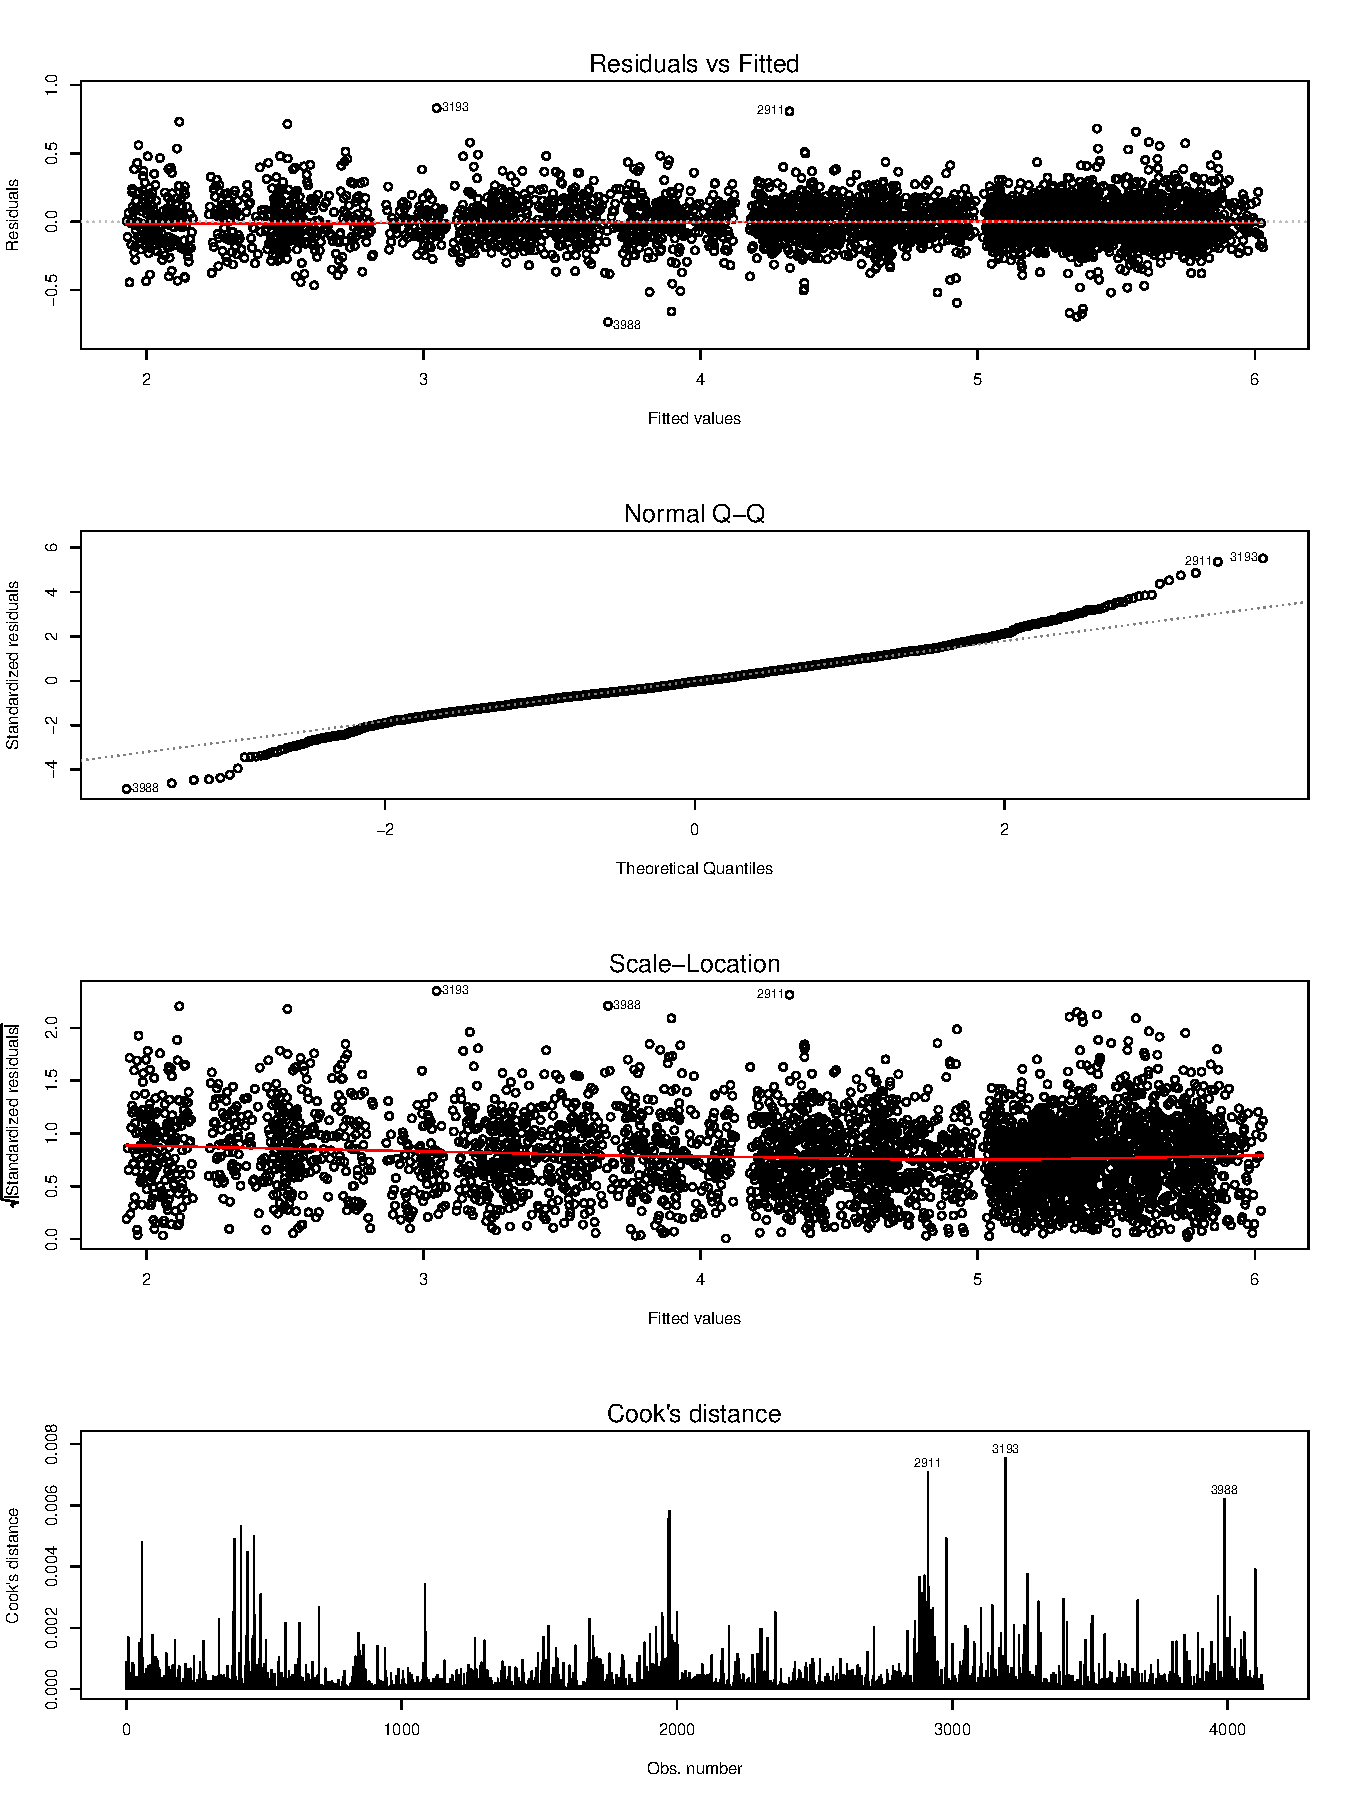
\includegraphics[width=\textwidth]{../plots/fit-assumptions}    
    \caption{Plots for confirming model assumptions.}    
    \label{fit-assumptions}
\end{figure}
\clearpage



\clearpage

\begin{figure}[!ht]
    \center
    % !TEX encoding = UTF-8 Unicode
\begin{tikzpicture}[x=1pt,y=1pt]
\definecolor{fillColor}{RGB}{255,255,255}
\path[use as bounding box,fill=fillColor,fill opacity=0.00] (0,0) rectangle (433.62,216.81);
\begin{scope}
\path[clip] (  0.00,  0.00) rectangle (433.62,216.81);
\definecolor{drawColor}{RGB}{255,255,255}
\definecolor{fillColor}{RGB}{255,255,255}

\path[draw=drawColor,line width= 0.6pt,line join=round,line cap=round,fill=fillColor] (  0.00,  0.00) rectangle (433.62,216.81);
\end{scope}
\begin{scope}
\path[clip] ( 48.27, 34.62) rectangle (427.62,210.81);
\definecolor{fillColor}{RGB}{255,255,255}

\path[fill=fillColor] ( 48.27, 34.62) rectangle (427.62,210.81);
\definecolor{drawColor}{gray}{0.98}

\path[draw=drawColor,line width= 0.6pt,line join=round] ( 48.27, 71.65) --
	(427.62, 71.65);

\path[draw=drawColor,line width= 0.6pt,line join=round] ( 48.27,112.32) --
	(427.62,112.32);

\path[draw=drawColor,line width= 0.6pt,line join=round] ( 48.27,152.99) --
	(427.62,152.99);

\path[draw=drawColor,line width= 0.6pt,line join=round] ( 48.27,193.66) --
	(427.62,193.66);

\path[draw=drawColor,line width= 0.6pt,line join=round] ( 66.44, 34.62) --
	( 66.44,210.81);

\path[draw=drawColor,line width= 0.6pt,line join=round] (115.74, 34.62) --
	(115.74,210.81);

\path[draw=drawColor,line width= 0.6pt,line join=round] (165.03, 34.62) --
	(165.03,210.81);

\path[draw=drawColor,line width= 0.6pt,line join=round] (214.33, 34.62) --
	(214.33,210.81);

\path[draw=drawColor,line width= 0.6pt,line join=round] (263.62, 34.62) --
	(263.62,210.81);

\path[draw=drawColor,line width= 0.6pt,line join=round] (312.92, 34.62) --
	(312.92,210.81);

\path[draw=drawColor,line width= 0.6pt,line join=round] (362.21, 34.62) --
	(362.21,210.81);

\path[draw=drawColor,line width= 0.6pt,line join=round] (411.51, 34.62) --
	(411.51,210.81);
\definecolor{drawColor}{gray}{0.90}

\path[draw=drawColor,line width= 0.2pt,line join=round] ( 48.27, 51.32) --
	(427.62, 51.32);

\path[draw=drawColor,line width= 0.2pt,line join=round] ( 48.27, 91.99) --
	(427.62, 91.99);

\path[draw=drawColor,line width= 0.2pt,line join=round] ( 48.27,132.66) --
	(427.62,132.66);

\path[draw=drawColor,line width= 0.2pt,line join=round] ( 48.27,173.33) --
	(427.62,173.33);

\path[draw=drawColor,line width= 0.2pt,line join=round] ( 91.09, 34.62) --
	( 91.09,210.81);

\path[draw=drawColor,line width= 0.2pt,line join=round] (140.38, 34.62) --
	(140.38,210.81);

\path[draw=drawColor,line width= 0.2pt,line join=round] (189.68, 34.62) --
	(189.68,210.81);

\path[draw=drawColor,line width= 0.2pt,line join=round] (238.97, 34.62) --
	(238.97,210.81);

\path[draw=drawColor,line width= 0.2pt,line join=round] (288.27, 34.62) --
	(288.27,210.81);

\path[draw=drawColor,line width= 0.2pt,line join=round] (337.56, 34.62) --
	(337.56,210.81);

\path[draw=drawColor,line width= 0.2pt,line join=round] (386.86, 34.62) --
	(386.86,210.81);
\definecolor{fillColor}{gray}{0.35}

\path[fill=fillColor] ( 65.52,132.66) rectangle ( 67.37,156.89);

\path[fill=fillColor] ( 67.57,132.66) rectangle ( 69.42,186.86);

\path[fill=fillColor] ( 69.62, 59.65) rectangle ( 71.47,132.66);

\path[fill=fillColor] ( 71.68,132.66) rectangle ( 73.53,193.17);

\path[fill=fillColor] ( 73.73,132.66) rectangle ( 75.58,202.80);

\path[fill=fillColor] ( 75.79,132.66) rectangle ( 77.64,155.19);

\path[fill=fillColor] ( 77.84,132.66) rectangle ( 79.69,169.25);

\path[fill=fillColor] ( 79.89,132.66) rectangle ( 81.74,166.79);

\path[fill=fillColor] ( 81.95,132.66) rectangle ( 83.80,191.21);

\path[fill=fillColor] ( 84.00,132.66) rectangle ( 85.85,166.50);

\path[fill=fillColor] ( 86.06,132.66) rectangle ( 87.90,162.16);

\path[fill=fillColor] ( 88.11,132.66) rectangle ( 89.96,145.85);

\path[fill=fillColor] ( 90.16,132.66) rectangle ( 92.01,150.30);

\path[fill=fillColor] ( 92.22,132.66) rectangle ( 94.07,156.16);

\path[fill=fillColor] ( 94.27,132.66) rectangle ( 96.12,141.57);

\path[fill=fillColor] ( 96.33,132.66) rectangle ( 98.17,150.97);

\path[fill=fillColor] ( 98.38,132.66) rectangle (100.23,147.87);

\path[fill=fillColor] (100.43,132.66) rectangle (102.28,136.06);

\path[fill=fillColor] (102.49,132.66) rectangle (104.34,141.55);

\path[fill=fillColor] (104.54,132.66) rectangle (106.39,153.65);

\path[fill=fillColor] (106.60,104.49) rectangle (108.44,132.66);

\path[fill=fillColor] (108.65,132.66) rectangle (110.50,133.93);

\path[fill=fillColor] (110.70,123.73) rectangle (112.55,132.66);

\path[fill=fillColor] (112.76,129.61) rectangle (114.61,132.66);

\path[fill=fillColor] (114.81, 66.76) rectangle (116.66,132.66);

\path[fill=fillColor] (116.87,132.66) rectangle (118.71,147.49);

\path[fill=fillColor] (118.92,132.66) rectangle (120.77,134.49);

\path[fill=fillColor] (120.97,132.66) rectangle (122.82,164.41);

\path[fill=fillColor] (123.03,117.79) rectangle (124.88,132.66);

\path[fill=fillColor] (125.08,103.11) rectangle (126.93,132.66);

\path[fill=fillColor] (127.14,123.20) rectangle (128.98,132.66);

\path[fill=fillColor] (129.19,127.50) rectangle (131.04,132.66);

\path[fill=fillColor] (131.24, 98.30) rectangle (133.09,132.66);

\path[fill=fillColor] (133.30,127.33) rectangle (135.15,132.66);

\path[fill=fillColor] (135.35,131.85) rectangle (137.20,132.66);

\path[fill=fillColor] (137.41,128.69) rectangle (139.25,132.66);

\path[fill=fillColor] (139.46,112.69) rectangle (141.31,132.66);

\path[fill=fillColor] (141.51,103.73) rectangle (143.36,132.66);

\path[fill=fillColor] (143.57, 96.95) rectangle (145.42,132.66);

\path[fill=fillColor] (145.62,107.93) rectangle (147.47,132.66);

\path[fill=fillColor] (147.68,111.88) rectangle (149.52,132.66);

\path[fill=fillColor] (149.73,117.58) rectangle (151.58,132.66);

\path[fill=fillColor] (151.78,120.76) rectangle (153.63,132.66);

\path[fill=fillColor] (153.84,132.66) rectangle (155.69,133.66);

\path[fill=fillColor] (155.89,126.49) rectangle (157.74,132.66);

\path[fill=fillColor] (157.94,126.19) rectangle (159.79,132.66);

\path[fill=fillColor] (160.00, 52.15) rectangle (161.85,132.66);

\path[fill=fillColor] (162.05, 42.63) rectangle (163.90,132.66);

\path[fill=fillColor] (164.11, 76.08) rectangle (165.96,132.66);

\path[fill=fillColor] (166.16, 49.05) rectangle (168.01,132.66);

\path[fill=fillColor] (168.21, 73.54) rectangle (170.06,132.66);

\path[fill=fillColor] (170.27,125.00) rectangle (172.12,132.66);

\path[fill=fillColor] (172.32,121.88) rectangle (174.17,132.66);

\path[fill=fillColor] (174.38,112.84) rectangle (176.23,132.66);

\path[fill=fillColor] (176.43, 97.50) rectangle (178.28,132.66);

\path[fill=fillColor] (178.48,117.48) rectangle (180.33,132.66);

\path[fill=fillColor] (180.54,124.81) rectangle (182.39,132.66);

\path[fill=fillColor] (182.59, 87.63) rectangle (184.44,132.66);

\path[fill=fillColor] (184.65,107.42) rectangle (186.50,132.66);

\path[fill=fillColor] (186.70,104.52) rectangle (188.55,132.66);

\path[fill=fillColor] (188.75,104.30) rectangle (190.60,132.66);

\path[fill=fillColor] (190.81, 91.03) rectangle (192.66,132.66);

\path[fill=fillColor] (192.86,120.62) rectangle (194.71,132.66);

\path[fill=fillColor] (194.92, 95.47) rectangle (196.76,132.66);

\path[fill=fillColor] (196.97, 95.65) rectangle (198.82,132.66);

\path[fill=fillColor] (199.02, 94.84) rectangle (200.87,132.66);

\path[fill=fillColor] (201.08,118.75) rectangle (202.93,132.66);

\path[fill=fillColor] (203.13,132.66) rectangle (204.98,137.49);

\path[fill=fillColor] (205.19, 94.72) rectangle (207.03,132.66);

\path[fill=fillColor] (207.24, 91.37) rectangle (209.09,132.66);

\path[fill=fillColor] (209.29,131.74) rectangle (211.14,132.66);

\path[fill=fillColor] (211.35, 84.73) rectangle (213.20,132.66);

\path[fill=fillColor] (213.40, 73.40) rectangle (215.25,132.66);

\path[fill=fillColor] (215.46, 70.64) rectangle (217.30,132.66);

\path[fill=fillColor] (217.51, 80.77) rectangle (219.36,132.66);

\path[fill=fillColor] (219.56,125.81) rectangle (221.41,132.66);

\path[fill=fillColor] (221.62, 88.10) rectangle (223.47,132.66);

\path[fill=fillColor] (223.67,117.00) rectangle (225.52,132.66);

\path[fill=fillColor] (225.73,132.66) rectangle (227.57,138.89);

\path[fill=fillColor] (227.78,109.99) rectangle (229.63,132.66);

\path[fill=fillColor] (229.83,119.50) rectangle (231.68,132.66);

\path[fill=fillColor] (231.89,107.58) rectangle (233.74,132.66);

\path[fill=fillColor] (233.94,124.61) rectangle (235.79,132.66);

\path[fill=fillColor] (236.00,126.89) rectangle (237.84,132.66);

\path[fill=fillColor] (238.05,132.66) rectangle (239.90,133.51);

\path[fill=fillColor] (240.10,119.89) rectangle (241.95,132.66);

\path[fill=fillColor] (242.16,132.66) rectangle (244.01,133.43);

\path[fill=fillColor] (244.21,108.94) rectangle (246.06,132.66);

\path[fill=fillColor] (246.27,109.55) rectangle (248.11,132.66);

\path[fill=fillColor] (248.32,113.09) rectangle (250.17,132.66);

\path[fill=fillColor] (250.37,118.73) rectangle (252.22,132.66);

\path[fill=fillColor] (252.43,116.62) rectangle (254.28,132.66);

\path[fill=fillColor] (254.48,119.68) rectangle (256.33,132.66);

\path[fill=fillColor] (256.54,121.23) rectangle (258.38,132.66);

\path[fill=fillColor] (258.59,117.51) rectangle (260.44,132.66);

\path[fill=fillColor] (260.64, 72.47) rectangle (262.49,132.66);

\path[fill=fillColor] (262.70, 53.83) rectangle (264.55,132.66);

\path[fill=fillColor] (264.75,132.66) rectangle (266.60,158.10);

\path[fill=fillColor] (266.80,110.99) rectangle (268.65,132.66);

\path[fill=fillColor] (268.86,132.66) rectangle (270.71,150.89);

\path[fill=fillColor] (270.91, 90.46) rectangle (272.76,132.66);

\path[fill=fillColor] (272.97,125.48) rectangle (274.82,132.66);

\path[fill=fillColor] (275.02,112.14) rectangle (276.87,132.66);

\path[fill=fillColor] (277.07,118.21) rectangle (278.92,132.66);

\path[fill=fillColor] (279.13,110.07) rectangle (280.98,132.66);

\path[fill=fillColor] (281.18, 97.51) rectangle (283.03,132.66);

\path[fill=fillColor] (283.24,111.79) rectangle (285.09,132.66);

\path[fill=fillColor] (285.29,114.43) rectangle (287.14,132.66);

\path[fill=fillColor] (287.34,114.66) rectangle (289.19,132.66);

\path[fill=fillColor] (289.40,112.67) rectangle (291.25,132.66);

\path[fill=fillColor] (291.45,122.27) rectangle (293.30,132.66);

\path[fill=fillColor] (293.51,123.57) rectangle (295.36,132.66);

\path[fill=fillColor] (295.56,104.81) rectangle (297.41,132.66);

\path[fill=fillColor] (297.61,107.72) rectangle (299.46,132.66);

\path[fill=fillColor] (299.67,132.66) rectangle (301.52,136.12);

\path[fill=fillColor] (301.72,132.37) rectangle (303.57,132.66);

\path[fill=fillColor] (303.78,127.95) rectangle (305.62,132.66);

\path[fill=fillColor] (305.83,102.68) rectangle (307.68,132.66);

\path[fill=fillColor] (307.88, 92.70) rectangle (309.73,132.66);

\path[fill=fillColor] (309.94,124.22) rectangle (311.79,132.66);

\path[fill=fillColor] (311.99, 86.99) rectangle (313.84,132.66);

\path[fill=fillColor] (314.05, 91.18) rectangle (315.89,132.66);

\path[fill=fillColor] (316.10,107.20) rectangle (317.95,132.66);

\path[fill=fillColor] (318.15,132.66) rectangle (320.00,163.18);

\path[fill=fillColor] (320.21,132.66) rectangle (322.06,135.92);

\path[fill=fillColor] (322.26,132.66) rectangle (324.11,155.27);

\path[fill=fillColor] (324.32,132.66) rectangle (326.16,165.13);

\path[fill=fillColor] (326.37,132.66) rectangle (328.22,188.30);

\path[fill=fillColor] (328.42,129.57) rectangle (330.27,132.66);

\path[fill=fillColor] (330.48,131.31) rectangle (332.33,132.66);

\path[fill=fillColor] (332.53,122.90) rectangle (334.38,132.66);

\path[fill=fillColor] (334.59,125.08) rectangle (336.43,132.66);

\path[fill=fillColor] (336.64,132.66) rectangle (338.49,151.27);

\path[fill=fillColor] (338.69,121.06) rectangle (340.54,132.66);

\path[fill=fillColor] (340.75,114.50) rectangle (342.60,132.66);

\path[fill=fillColor] (342.80,115.69) rectangle (344.65,132.66);

\path[fill=fillColor] (344.86,127.26) rectangle (346.70,132.66);

\path[fill=fillColor] (346.91,124.08) rectangle (348.76,132.66);

\path[fill=fillColor] (348.96,120.10) rectangle (350.81,132.66);

\path[fill=fillColor] (351.02,132.66) rectangle (352.87,156.70);

\path[fill=fillColor] (353.07,111.89) rectangle (354.92,132.66);

\path[fill=fillColor] (355.13, 95.23) rectangle (356.97,132.66);

\path[fill=fillColor] (357.18,132.66) rectangle (359.03,144.95);

\path[fill=fillColor] (359.23,132.66) rectangle (361.08,164.22);

\path[fill=fillColor] (361.29,132.66) rectangle (363.14,151.51);

\path[fill=fillColor] (363.34,123.26) rectangle (365.19,132.66);

\path[fill=fillColor] (365.40,102.27) rectangle (367.24,132.66);

\path[fill=fillColor] (367.45,123.47) rectangle (369.30,132.66);

\path[fill=fillColor] (369.50,132.66) rectangle (371.35,153.82);

\path[fill=fillColor] (371.56,132.66) rectangle (373.41,144.21);

\path[fill=fillColor] (373.61,132.66) rectangle (375.46,150.22);

\path[fill=fillColor] (375.67,132.66) rectangle (377.51,136.02);

\path[fill=fillColor] (377.72,132.66) rectangle (379.57,150.46);

\path[fill=fillColor] (379.77,132.66) rectangle (381.62,140.03);

\path[fill=fillColor] (381.83,122.54) rectangle (383.68,132.66);

\path[fill=fillColor] (383.88,127.05) rectangle (385.73,132.66);

\path[fill=fillColor] (385.93,113.86) rectangle (387.78,132.66);

\path[fill=fillColor] (387.99,110.84) rectangle (389.84,132.66);

\path[fill=fillColor] (390.04,132.66) rectangle (391.89,138.96);

\path[fill=fillColor] (392.10,116.44) rectangle (393.95,132.66);

\path[fill=fillColor] (394.15,124.26) rectangle (396.00,132.66);

\path[fill=fillColor] (396.20,121.17) rectangle (398.05,132.66);

\path[fill=fillColor] (398.26,132.64) rectangle (400.11,132.66);

\path[fill=fillColor] (400.31,131.93) rectangle (402.16,132.66);

\path[fill=fillColor] (402.37,132.66) rectangle (404.22,136.40);

\path[fill=fillColor] (404.42, 83.80) rectangle (406.27,132.66);

\path[fill=fillColor] (406.47, 93.36) rectangle (408.32,132.66);

\path[fill=fillColor] (408.53,120.94) rectangle (410.38,132.66);
\definecolor{drawColor}{gray}{0.50}

\path[draw=drawColor,line width= 0.6pt,line join=round,line cap=round] ( 48.27, 34.62) rectangle (427.62,210.81);
\end{scope}
\begin{scope}
\path[clip] (  0.00,  0.00) rectangle (433.62,216.81);
\definecolor{drawColor}{RGB}{0,0,0}

\node[text=drawColor,anchor=base east,inner sep=0pt, outer sep=0pt, scale=  0.96] at ( 42.87, 48.01) {-0.50};

\node[text=drawColor,anchor=base east,inner sep=0pt, outer sep=0pt, scale=  0.96] at ( 42.87, 88.68) {-0.25};

\node[text=drawColor,anchor=base east,inner sep=0pt, outer sep=0pt, scale=  0.96] at ( 42.87,129.35) {0.00};

\node[text=drawColor,anchor=base east,inner sep=0pt, outer sep=0pt, scale=  0.96] at ( 42.87,170.02) {0.25};
\end{scope}
\begin{scope}
\path[clip] (  0.00,  0.00) rectangle (433.62,216.81);
\definecolor{drawColor}{RGB}{0,0,0}

\path[draw=drawColor,line width= 0.6pt,line join=round] ( 45.27, 51.32) --
	( 48.27, 51.32);

\path[draw=drawColor,line width= 0.6pt,line join=round] ( 45.27, 91.99) --
	( 48.27, 91.99);

\path[draw=drawColor,line width= 0.6pt,line join=round] ( 45.27,132.66) --
	( 48.27,132.66);

\path[draw=drawColor,line width= 0.6pt,line join=round] ( 45.27,173.33) --
	( 48.27,173.33);
\end{scope}
\begin{scope}
\path[clip] (  0.00,  0.00) rectangle (433.62,216.81);
\definecolor{drawColor}{RGB}{0,0,0}

\path[draw=drawColor,line width= 0.6pt,line join=round] ( 91.09, 31.62) --
	( 91.09, 34.62);

\path[draw=drawColor,line width= 0.6pt,line join=round] (140.38, 31.62) --
	(140.38, 34.62);

\path[draw=drawColor,line width= 0.6pt,line join=round] (189.68, 31.62) --
	(189.68, 34.62);

\path[draw=drawColor,line width= 0.6pt,line join=round] (238.97, 31.62) --
	(238.97, 34.62);

\path[draw=drawColor,line width= 0.6pt,line join=round] (288.27, 31.62) --
	(288.27, 34.62);

\path[draw=drawColor,line width= 0.6pt,line join=round] (337.56, 31.62) --
	(337.56, 34.62);

\path[draw=drawColor,line width= 0.6pt,line join=round] (386.86, 31.62) --
	(386.86, 34.62);
\end{scope}
\begin{scope}
\path[clip] (  0.00,  0.00) rectangle (433.62,216.81);
\definecolor{drawColor}{RGB}{0,0,0}

\node[text=drawColor,anchor=base,inner sep=0pt, outer sep=0pt, scale=  0.96] at ( 91.09, 22.61) {Mon};

\node[text=drawColor,anchor=base,inner sep=0pt, outer sep=0pt, scale=  0.96] at (140.38, 22.61) {Tue};

\node[text=drawColor,anchor=base,inner sep=0pt, outer sep=0pt, scale=  0.96] at (189.68, 22.61) {Wed};

\node[text=drawColor,anchor=base,inner sep=0pt, outer sep=0pt, scale=  0.96] at (238.97, 22.61) {Thu};

\node[text=drawColor,anchor=base,inner sep=0pt, outer sep=0pt, scale=  0.96] at (288.27, 22.61) {Fri};

\node[text=drawColor,anchor=base,inner sep=0pt, outer sep=0pt, scale=  0.96] at (337.56, 22.61) {Sat};

\node[text=drawColor,anchor=base,inner sep=0pt, outer sep=0pt, scale=  0.96] at (386.86, 22.61) {Sun};
\end{scope}
\begin{scope}
\path[clip] (  0.00,  0.00) rectangle (433.62,216.81);
\definecolor{drawColor}{RGB}{0,0,0}

\node[text=drawColor,anchor=base,inner sep=0pt, outer sep=0pt, scale=  0.96] at (237.95,  6.00) {DateTime};
\end{scope}
\begin{scope}
\path[clip] (  0.00,  0.00) rectangle (433.62,216.81);
\definecolor{drawColor}{RGB}{0,0,0}

\node[text=drawColor,rotate= 90.00,anchor=base,inner sep=0pt, outer sep=0pt, scale=  0.96] at ( 12.61,122.72) {Error/CheckInCount};
\end{scope}
\end{tikzpicture}

    \caption{Error percentage of a single week.}
    \label{fig:travelcard_error_pct}
\end{figure}

\begin{figure}[!ht]
    \center
    % !TEX encoding = UTF-8 Unicode
\begin{tikzpicture}[x=1pt,y=1pt]
\definecolor{fillColor}{RGB}{255,255,255}
\path[use as bounding box,fill=fillColor,fill opacity=0.00] (0,0) rectangle (433.62,216.81);
\begin{scope}
\path[clip] (  0.00,  0.00) rectangle (433.62,216.81);
\definecolor{drawColor}{RGB}{255,255,255}
\definecolor{fillColor}{RGB}{255,255,255}

\path[draw=drawColor,line width= 0.6pt,line join=round,line cap=round,fill=fillColor] (  0.00,  0.00) rectangle (433.62,216.81);
\end{scope}
\begin{scope}
\path[clip] ( 32.81, 34.62) rectangle (427.62,210.81);
\definecolor{fillColor}{RGB}{255,255,255}

\path[fill=fillColor] ( 32.81, 34.62) rectangle (427.62,210.81);
\definecolor{drawColor}{gray}{0.98}

\path[draw=drawColor,line width= 0.6pt,line join=round] ( 32.81, 69.33) --
	(427.62, 69.33);

\path[draw=drawColor,line width= 0.6pt,line join=round] ( 32.81,122.72) --
	(427.62,122.72);

\path[draw=drawColor,line width= 0.6pt,line join=round] ( 32.81,176.11) --
	(427.62,176.11);

\path[draw=drawColor,line width= 0.6pt,line join=round] ( 50.90, 34.62) --
	( 50.90,210.81);

\path[draw=drawColor,line width= 0.6pt,line join=round] (153.47, 34.62) --
	(153.47,210.81);

\path[draw=drawColor,line width= 0.6pt,line join=round] (256.04, 34.62) --
	(256.04,210.81);

\path[draw=drawColor,line width= 0.6pt,line join=round] (358.60, 34.62) --
	(358.60,210.81);
\definecolor{drawColor}{gray}{0.90}

\path[draw=drawColor,line width= 0.2pt,line join=round] ( 32.81, 42.63) --
	(427.62, 42.63);

\path[draw=drawColor,line width= 0.2pt,line join=round] ( 32.81, 96.02) --
	(427.62, 96.02);

\path[draw=drawColor,line width= 0.2pt,line join=round] ( 32.81,149.41) --
	(427.62,149.41);

\path[draw=drawColor,line width= 0.2pt,line join=round] ( 32.81,202.80) --
	(427.62,202.80);

\path[draw=drawColor,line width= 0.2pt,line join=round] (102.18, 34.62) --
	(102.18,210.81);

\path[draw=drawColor,line width= 0.2pt,line join=round] (204.75, 34.62) --
	(204.75,210.81);

\path[draw=drawColor,line width= 0.2pt,line join=round] (307.32, 34.62) --
	(307.32,210.81);

\path[draw=drawColor,line width= 0.2pt,line join=round] (409.89, 34.62) --
	(409.89,210.81);
\definecolor{fillColor}{RGB}{0,0,255}

\path[fill=fillColor] ( 50.76, 42.63) rectangle ( 51.04, 96.02);

\path[fill=fillColor] ( 51.47, 42.63) rectangle ( 51.76, 69.33);

\path[fill=fillColor] ( 52.54, 42.63) rectangle ( 52.83, 69.33);

\path[fill=fillColor] ( 52.89, 42.63) rectangle ( 53.18, 96.02);

\path[fill=fillColor] ( 53.61, 42.63) rectangle ( 53.89, 69.33);

\path[fill=fillColor] ( 54.67, 42.63) rectangle ( 54.96,122.72);

\path[fill=fillColor] ( 55.03, 42.63) rectangle ( 55.32,122.72);

\path[fill=fillColor] ( 55.74, 42.63) rectangle ( 56.03,122.72);

\path[fill=fillColor] ( 56.81, 42.63) rectangle ( 57.10, 69.33);

\path[fill=fillColor] ( 57.17, 42.63) rectangle ( 57.46, 69.33);

\path[fill=fillColor] ( 57.88, 42.63) rectangle ( 58.17, 69.33);

\path[fill=fillColor] ( 58.95, 42.63) rectangle ( 59.24,176.11);

\path[fill=fillColor] ( 59.30, 42.63) rectangle ( 59.59,202.80);

\path[fill=fillColor] ( 60.02, 42.63) rectangle ( 60.30, 69.33);

\path[fill=fillColor] ( 61.08, 42.63) rectangle ( 61.37,122.72);

\path[fill=fillColor] ( 61.44, 42.63) rectangle ( 61.73,149.41);

\path[fill=fillColor] ( 62.15, 42.63) rectangle ( 62.44, 69.33);

\path[fill=fillColor] ( 63.22, 42.63) rectangle ( 63.51, 42.63);

\path[fill=fillColor] ( 63.58, 42.63) rectangle ( 63.87,149.41);

\path[fill=fillColor] ( 64.29, 42.63) rectangle ( 64.58, 42.63);

\path[fill=fillColor] ( 65.36, 42.63) rectangle ( 65.65, 42.63);

\path[fill=fillColor] ( 65.71, 42.63) rectangle ( 66.00, 42.63);

\path[fill=fillColor] ( 66.43, 42.63) rectangle ( 66.71, 42.63);

\path[fill=fillColor] ( 67.49, 42.63) rectangle ( 67.78, 42.63);

\path[fill=fillColor] ( 67.85, 42.63) rectangle ( 68.14, 42.63);

\path[fill=fillColor] ( 68.56, 42.63) rectangle ( 68.85,122.72);

\path[fill=fillColor] ( 69.63, 42.63) rectangle ( 69.92,122.72);

\path[fill=fillColor] ( 69.99, 42.63) rectangle ( 70.28, 96.02);

\path[fill=fillColor] ( 70.70, 42.63) rectangle ( 70.99,122.72);

\path[fill=fillColor] ( 71.77, 42.63) rectangle ( 72.06, 69.33);

\path[fill=fillColor] ( 72.12, 42.63) rectangle ( 72.41, 96.02);

\path[fill=fillColor] ( 72.84, 42.63) rectangle ( 73.13, 69.33);

\path[fill=fillColor] ( 73.91, 42.63) rectangle ( 74.19, 42.63);

\path[fill=fillColor] ( 74.26, 42.63) rectangle ( 74.55, 69.33);

\path[fill=fillColor] ( 74.97, 42.63) rectangle ( 75.26, 69.33);

\path[fill=fillColor] ( 76.04, 42.63) rectangle ( 76.33, 69.33);

\path[fill=fillColor] ( 76.40, 42.63) rectangle ( 76.69, 69.33);

\path[fill=fillColor] ( 77.11, 42.63) rectangle ( 77.40, 42.63);

\path[fill=fillColor] ( 78.18, 42.63) rectangle ( 78.47, 42.63);

\path[fill=fillColor] ( 78.54, 42.63) rectangle ( 78.82, 42.63);

\path[fill=fillColor] ( 79.25, 42.63) rectangle ( 79.54, 42.63);

\path[fill=fillColor] ( 80.32, 42.63) rectangle ( 80.60, 42.63);

\path[fill=fillColor] ( 80.67, 42.63) rectangle ( 80.96, 42.63);

\path[fill=fillColor] ( 81.38, 42.63) rectangle ( 81.67, 42.63);

\path[fill=fillColor] ( 82.45, 42.63) rectangle ( 82.74, 42.63);

\path[fill=fillColor] ( 82.81, 42.63) rectangle ( 83.10, 42.63);

\path[fill=fillColor] ( 83.52, 42.63) rectangle ( 83.81, 42.63);

\path[fill=fillColor] ( 84.59, 42.63) rectangle ( 84.88, 42.63);

\path[fill=fillColor] ( 84.95, 42.63) rectangle ( 85.23, 42.63);

\path[fill=fillColor] ( 85.66, 42.63) rectangle ( 85.95, 42.63);

\path[fill=fillColor] ( 86.73, 42.63) rectangle ( 87.01, 42.63);

\path[fill=fillColor] ( 87.08, 42.63) rectangle ( 87.37, 42.63);

\path[fill=fillColor] ( 87.79, 42.63) rectangle ( 88.08, 42.63);

\path[fill=fillColor] ( 88.86, 42.63) rectangle ( 89.15, 42.63);

\path[fill=fillColor] ( 89.22, 42.63) rectangle ( 89.51, 42.63);

\path[fill=fillColor] ( 89.93, 42.63) rectangle ( 90.22, 42.63);

\path[fill=fillColor] ( 91.00, 42.63) rectangle ( 91.29, 42.63);

\path[fill=fillColor] ( 91.36, 42.63) rectangle ( 91.64, 42.63);

\path[fill=fillColor] ( 92.07, 42.63) rectangle ( 92.36, 42.63);

\path[fill=fillColor] ( 93.14, 42.63) rectangle ( 93.43, 42.63);

\path[fill=fillColor] ( 93.49, 42.63) rectangle ( 93.78, 42.63);

\path[fill=fillColor] ( 94.21, 42.63) rectangle ( 94.49, 42.63);

\path[fill=fillColor] ( 95.27, 42.63) rectangle ( 95.56, 42.63);

\path[fill=fillColor] ( 95.63, 42.63) rectangle ( 95.92, 42.63);

\path[fill=fillColor] ( 96.34, 42.63) rectangle ( 96.63, 42.63);

\path[fill=fillColor] ( 97.41, 42.63) rectangle ( 97.70, 42.63);

\path[fill=fillColor] ( 97.77, 42.63) rectangle ( 98.05, 42.63);

\path[fill=fillColor] ( 98.48, 42.63) rectangle ( 98.77, 42.63);

\path[fill=fillColor] ( 99.55, 42.63) rectangle ( 99.84, 42.63);

\path[fill=fillColor] ( 99.90, 42.63) rectangle (100.19, 42.63);

\path[fill=fillColor] (100.62, 42.63) rectangle (100.90, 42.63);

\path[fill=fillColor] (101.68, 42.63) rectangle (101.97, 42.63);

\path[fill=fillColor] (102.04, 42.63) rectangle (102.33, 42.63);

\path[fill=fillColor] (102.75, 42.63) rectangle (103.04, 42.63);

\path[fill=fillColor] (103.82, 42.63) rectangle (104.11, 42.63);

\path[fill=fillColor] (104.18, 42.63) rectangle (104.47, 42.63);

\path[fill=fillColor] (104.89, 42.63) rectangle (105.18, 42.63);

\path[fill=fillColor] (105.96, 42.63) rectangle (106.25, 42.63);

\path[fill=fillColor] (106.31, 42.63) rectangle (106.60, 42.63);

\path[fill=fillColor] (107.03, 42.63) rectangle (107.31, 42.63);

\path[fill=fillColor] (108.09, 42.63) rectangle (108.38, 42.63);

\path[fill=fillColor] (108.45, 42.63) rectangle (108.74, 42.63);

\path[fill=fillColor] (109.16, 42.63) rectangle (109.45, 42.63);

\path[fill=fillColor] (110.23, 42.63) rectangle (110.52, 42.63);

\path[fill=fillColor] (110.59, 42.63) rectangle (110.88, 42.63);

\path[fill=fillColor] (111.30, 42.63) rectangle (111.59, 42.63);

\path[fill=fillColor] (112.37, 42.63) rectangle (112.66, 42.63);

\path[fill=fillColor] (112.72, 42.63) rectangle (113.01, 42.63);

\path[fill=fillColor] (113.44, 42.63) rectangle (113.72, 42.63);

\path[fill=fillColor] (114.50, 42.63) rectangle (114.79, 42.63);

\path[fill=fillColor] (114.86, 42.63) rectangle (115.15, 42.63);

\path[fill=fillColor] (115.57, 42.63) rectangle (115.86, 42.63);

\path[fill=fillColor] (116.64, 42.63) rectangle (116.93, 42.63);

\path[fill=fillColor] (117.00, 42.63) rectangle (117.29, 42.63);

\path[fill=fillColor] (117.71, 42.63) rectangle (118.00, 42.63);

\path[fill=fillColor] (118.78, 42.63) rectangle (119.07, 42.63);

\path[fill=fillColor] (119.13, 42.63) rectangle (119.42, 42.63);

\path[fill=fillColor] (119.85, 42.63) rectangle (120.14, 42.63);

\path[fill=fillColor] (120.92, 42.63) rectangle (121.20, 42.63);

\path[fill=fillColor] (121.27, 42.63) rectangle (121.56, 42.63);

\path[fill=fillColor] (121.98, 42.63) rectangle (122.27, 42.63);

\path[fill=fillColor] (123.05, 42.63) rectangle (123.34, 42.63);

\path[fill=fillColor] (123.41, 42.63) rectangle (123.70, 42.63);

\path[fill=fillColor] (124.12, 42.63) rectangle (124.41, 42.63);

\path[fill=fillColor] (125.19, 42.63) rectangle (125.48, 42.63);

\path[fill=fillColor] (125.55, 42.63) rectangle (125.83, 42.63);

\path[fill=fillColor] (126.26, 42.63) rectangle (126.55, 42.63);

\path[fill=fillColor] (127.33, 42.63) rectangle (127.61, 42.63);

\path[fill=fillColor] (127.68, 42.63) rectangle (127.97, 69.33);

\path[fill=fillColor] (128.39, 42.63) rectangle (128.68, 42.63);

\path[fill=fillColor] (129.46, 42.63) rectangle (129.75, 42.63);

\path[fill=fillColor] (129.82, 42.63) rectangle (130.11, 42.63);

\path[fill=fillColor] (130.53, 42.63) rectangle (130.82, 42.63);

\path[fill=fillColor] (131.60, 42.63) rectangle (131.89, 42.63);

\path[fill=fillColor] (131.96, 42.63) rectangle (132.24, 42.63);

\path[fill=fillColor] (132.67, 42.63) rectangle (132.96, 42.63);

\path[fill=fillColor] (133.74, 42.63) rectangle (134.02, 42.63);

\path[fill=fillColor] (134.09, 42.63) rectangle (134.38, 42.63);

\path[fill=fillColor] (135.87, 42.63) rectangle (136.16, 42.63);

\path[fill=fillColor] (136.23, 42.63) rectangle (136.52, 42.63);

\path[fill=fillColor] (136.94, 42.63) rectangle (137.23, 42.63);

\path[fill=fillColor] (138.01, 42.63) rectangle (138.30, 42.63);

\path[fill=fillColor] (138.37, 42.63) rectangle (138.65, 42.63);

\path[fill=fillColor] (139.08, 42.63) rectangle (139.37, 42.63);

\path[fill=fillColor] (140.15, 42.63) rectangle (140.44, 42.63);

\path[fill=fillColor] (140.50, 42.63) rectangle (140.79, 42.63);

\path[fill=fillColor] (141.22, 42.63) rectangle (141.50, 42.63);

\path[fill=fillColor] (142.28, 42.63) rectangle (142.57, 42.63);

\path[fill=fillColor] (142.64, 42.63) rectangle (142.93, 42.63);

\path[fill=fillColor] (143.35, 42.63) rectangle (143.64, 42.63);

\path[fill=fillColor] (144.42, 42.63) rectangle (144.71, 42.63);

\path[fill=fillColor] (144.78, 42.63) rectangle (145.06, 42.63);

\path[fill=fillColor] (145.49, 42.63) rectangle (145.78, 42.63);

\path[fill=fillColor] (146.56, 42.63) rectangle (146.85, 42.63);

\path[fill=fillColor] (146.91, 42.63) rectangle (147.20, 42.63);

\path[fill=fillColor] (147.63, 42.63) rectangle (147.91, 42.63);

\path[fill=fillColor] (148.69, 42.63) rectangle (148.98, 42.63);

\path[fill=fillColor] (149.05, 42.63) rectangle (149.34, 42.63);

\path[fill=fillColor] (149.76, 42.63) rectangle (150.05, 42.63);

\path[fill=fillColor] (150.83, 42.63) rectangle (151.12, 42.63);

\path[fill=fillColor] (151.19, 42.63) rectangle (151.48, 42.63);

\path[fill=fillColor] (151.90, 42.63) rectangle (152.19, 42.63);

\path[fill=fillColor] (152.97, 42.63) rectangle (153.26, 42.63);

\path[fill=fillColor] (153.32, 42.63) rectangle (153.61, 42.63);

\path[fill=fillColor] (154.04, 42.63) rectangle (154.32, 42.63);

\path[fill=fillColor] (155.10, 42.63) rectangle (155.39, 42.63);

\path[fill=fillColor] (155.46, 42.63) rectangle (155.75, 42.63);

\path[fill=fillColor] (156.17, 42.63) rectangle (156.46, 42.63);

\path[fill=fillColor] (157.24, 42.63) rectangle (157.53, 42.63);

\path[fill=fillColor] (157.60, 42.63) rectangle (157.89, 42.63);

\path[fill=fillColor] (158.31, 42.63) rectangle (158.60, 42.63);

\path[fill=fillColor] (159.38, 42.63) rectangle (159.67, 42.63);

\path[fill=fillColor] (159.73, 42.63) rectangle (160.02, 42.63);

\path[fill=fillColor] (160.45, 42.63) rectangle (160.73, 42.63);

\path[fill=fillColor] (161.51, 42.63) rectangle (161.80, 42.63);

\path[fill=fillColor] (161.87, 42.63) rectangle (162.16, 42.63);

\path[fill=fillColor] (162.58, 42.63) rectangle (162.87, 42.63);

\path[fill=fillColor] (163.65, 42.63) rectangle (163.94, 42.63);

\path[fill=fillColor] (164.01, 42.63) rectangle (164.30, 42.63);

\path[fill=fillColor] (164.72, 42.63) rectangle (165.01, 42.63);

\path[fill=fillColor] (165.79, 42.63) rectangle (166.08, 42.63);

\path[fill=fillColor] (166.14, 42.63) rectangle (166.43, 42.63);

\path[fill=fillColor] (166.86, 42.63) rectangle (167.15, 42.63);

\path[fill=fillColor] (167.93, 42.63) rectangle (168.21, 42.63);

\path[fill=fillColor] (168.28, 42.63) rectangle (168.57, 42.63);

\path[fill=fillColor] (168.99, 42.63) rectangle (169.28, 42.63);

\path[fill=fillColor] (170.06, 42.63) rectangle (170.35, 42.63);

\path[fill=fillColor] (170.42, 42.63) rectangle (170.71, 42.63);

\path[fill=fillColor] (171.13, 42.63) rectangle (171.42, 42.63);

\path[fill=fillColor] (172.20, 42.63) rectangle (172.49, 42.63);

\path[fill=fillColor] (172.56, 42.63) rectangle (172.84, 42.63);

\path[fill=fillColor] (173.27, 42.63) rectangle (173.56, 42.63);

\path[fill=fillColor] (174.34, 42.63) rectangle (174.62, 42.63);

\path[fill=fillColor] (174.69, 42.63) rectangle (174.98, 42.63);

\path[fill=fillColor] (175.40, 42.63) rectangle (175.69, 42.63);

\path[fill=fillColor] (176.47, 42.63) rectangle (176.76, 42.63);

\path[fill=fillColor] (178.97, 42.63) rectangle (179.25, 42.63);

\path[fill=fillColor] (179.68, 42.63) rectangle (179.97, 42.63);

\path[fill=fillColor] (180.75, 42.63) rectangle (181.03, 42.63);

\path[fill=fillColor] (181.10, 42.63) rectangle (181.39, 42.63);

\path[fill=fillColor] (181.81, 42.63) rectangle (182.10, 42.63);

\path[fill=fillColor] (182.88, 42.63) rectangle (183.17, 42.63);

\path[fill=fillColor] (183.24, 42.63) rectangle (183.53, 42.63);

\path[fill=fillColor] (183.95, 42.63) rectangle (184.24, 42.63);

\path[fill=fillColor] (185.02, 42.63) rectangle (185.31, 42.63);

\path[fill=fillColor] (185.38, 42.63) rectangle (185.66, 42.63);

\path[fill=fillColor] (186.09, 42.63) rectangle (186.38, 42.63);

\path[fill=fillColor] (187.16, 42.63) rectangle (187.45, 42.63);

\path[fill=fillColor] (187.51, 42.63) rectangle (187.80, 42.63);

\path[fill=fillColor] (188.23, 42.63) rectangle (188.51, 42.63);

\path[fill=fillColor] (189.29, 42.63) rectangle (189.58, 42.63);

\path[fill=fillColor] (189.65, 42.63) rectangle (189.94, 42.63);

\path[fill=fillColor] (190.36, 42.63) rectangle (190.65, 42.63);

\path[fill=fillColor] (191.43, 42.63) rectangle (191.72, 42.63);

\path[fill=fillColor] (191.79, 42.63) rectangle (192.07, 42.63);

\path[fill=fillColor] (192.50, 42.63) rectangle (192.79, 42.63);

\path[fill=fillColor] (193.57, 42.63) rectangle (193.86, 42.63);

\path[fill=fillColor] (193.92, 42.63) rectangle (194.21, 42.63);

\path[fill=fillColor] (194.64, 42.63) rectangle (194.92, 42.63);

\path[fill=fillColor] (195.70, 42.63) rectangle (195.99, 42.63);

\path[fill=fillColor] (196.06, 42.63) rectangle (196.35, 42.63);

\path[fill=fillColor] (196.77, 42.63) rectangle (197.06, 42.63);

\path[fill=fillColor] (197.84, 42.63) rectangle (198.13, 42.63);

\path[fill=fillColor] (198.20, 42.63) rectangle (198.49, 42.63);

\path[fill=fillColor] (198.91, 42.63) rectangle (199.20, 42.63);

\path[fill=fillColor] (199.98, 42.63) rectangle (200.27, 42.63);

\path[fill=fillColor] (200.33, 42.63) rectangle (200.62, 42.63);

\path[fill=fillColor] (201.05, 42.63) rectangle (201.33, 42.63);

\path[fill=fillColor] (202.11, 42.63) rectangle (202.40, 42.63);

\path[fill=fillColor] (202.47, 42.63) rectangle (202.76, 42.63);

\path[fill=fillColor] (203.18, 42.63) rectangle (203.47, 42.63);

\path[fill=fillColor] (204.25, 42.63) rectangle (204.54, 42.63);

\path[fill=fillColor] (204.61, 42.63) rectangle (204.90, 42.63);

\path[fill=fillColor] (205.32, 42.63) rectangle (205.61, 42.63);

\path[fill=fillColor] (206.39, 42.63) rectangle (206.68, 42.63);

\path[fill=fillColor] (206.74, 42.63) rectangle (207.03, 42.63);

\path[fill=fillColor] (207.46, 42.63) rectangle (207.74, 42.63);

\path[fill=fillColor] (208.52, 42.63) rectangle (208.81, 42.63);

\path[fill=fillColor] (208.88, 42.63) rectangle (209.17, 42.63);

\path[fill=fillColor] (209.59, 42.63) rectangle (209.88, 42.63);

\path[fill=fillColor] (210.66, 42.63) rectangle (210.95, 42.63);

\path[fill=fillColor] (211.02, 42.63) rectangle (211.31, 42.63);

\path[fill=fillColor] (211.73, 42.63) rectangle (212.02, 42.63);

\path[fill=fillColor] (212.80, 42.63) rectangle (213.09, 42.63);

\path[fill=fillColor] (213.15, 42.63) rectangle (213.44, 42.63);

\path[fill=fillColor] (213.87, 42.63) rectangle (214.16, 42.63);

\path[fill=fillColor] (214.94, 42.63) rectangle (215.22, 42.63);

\path[fill=fillColor] (215.29, 42.63) rectangle (215.58, 42.63);

\path[fill=fillColor] (216.00, 42.63) rectangle (216.29, 42.63);

\path[fill=fillColor] (217.07, 42.63) rectangle (217.36, 42.63);

\path[fill=fillColor] (217.43, 42.63) rectangle (217.72, 42.63);

\path[fill=fillColor] (218.14, 42.63) rectangle (218.43, 42.63);

\path[fill=fillColor] (219.21, 42.63) rectangle (219.50, 42.63);

\path[fill=fillColor] (219.57, 42.63) rectangle (219.85, 42.63);

\path[fill=fillColor] (220.28, 42.63) rectangle (220.57, 42.63);

\path[fill=fillColor] (221.35, 42.63) rectangle (221.63, 42.63);

\path[fill=fillColor] (221.70, 42.63) rectangle (221.99, 42.63);

\path[fill=fillColor] (222.41, 42.63) rectangle (222.70, 42.63);

\path[fill=fillColor] (223.48, 42.63) rectangle (223.77, 42.63);

\path[fill=fillColor] (223.84, 42.63) rectangle (224.13, 42.63);

\path[fill=fillColor] (224.55, 42.63) rectangle (224.84, 42.63);

\path[fill=fillColor] (225.62, 42.63) rectangle (225.91, 42.63);

\path[fill=fillColor] (225.98, 42.63) rectangle (226.26, 42.63);

\path[fill=fillColor] (226.69, 42.63) rectangle (226.98, 42.63);

\path[fill=fillColor] (227.76, 42.63) rectangle (228.04, 42.63);

\path[fill=fillColor] (228.11, 42.63) rectangle (228.40, 42.63);

\path[fill=fillColor] (228.82, 42.63) rectangle (229.11, 42.63);

\path[fill=fillColor] (229.89, 42.63) rectangle (230.18, 42.63);

\path[fill=fillColor] (230.25, 42.63) rectangle (230.54, 42.63);

\path[fill=fillColor] (230.96, 42.63) rectangle (231.25, 42.63);

\path[fill=fillColor] (232.03, 42.63) rectangle (232.32, 42.63);

\path[fill=fillColor] (232.39, 42.63) rectangle (232.67, 42.63);

\path[fill=fillColor] (233.10, 42.63) rectangle (233.39, 42.63);

\path[fill=fillColor] (234.17, 42.63) rectangle (234.46, 42.63);

\path[fill=fillColor] (234.52, 42.63) rectangle (234.81, 42.63);

\path[fill=fillColor] (235.24, 42.63) rectangle (235.52, 42.63);

\path[fill=fillColor] (236.30, 42.63) rectangle (236.59, 42.63);

\path[fill=fillColor] (236.66, 42.63) rectangle (236.95, 42.63);

\path[fill=fillColor] (237.37, 42.63) rectangle (237.66, 42.63);

\path[fill=fillColor] (238.44, 42.63) rectangle (238.73, 42.63);

\path[fill=fillColor] (238.80, 42.63) rectangle (239.08, 42.63);

\path[fill=fillColor] (239.51, 42.63) rectangle (239.80, 42.63);

\path[fill=fillColor] (240.58, 42.63) rectangle (240.87, 42.63);

\path[fill=fillColor] (240.93, 42.63) rectangle (241.22, 42.63);

\path[fill=fillColor] (241.65, 42.63) rectangle (241.93, 42.63);

\path[fill=fillColor] (242.71, 42.63) rectangle (243.00, 42.63);

\path[fill=fillColor] (243.07, 42.63) rectangle (243.36, 42.63);

\path[fill=fillColor] (243.78, 42.63) rectangle (244.07, 42.63);

\path[fill=fillColor] (244.85, 42.63) rectangle (245.14, 42.63);

\path[fill=fillColor] (245.21, 42.63) rectangle (245.50, 42.63);

\path[fill=fillColor] (245.92, 42.63) rectangle (246.21, 42.63);

\path[fill=fillColor] (246.99, 42.63) rectangle (247.28, 42.63);

\path[fill=fillColor] (247.34, 42.63) rectangle (247.63, 42.63);

\path[fill=fillColor] (248.06, 42.63) rectangle (248.34, 42.63);

\path[fill=fillColor] (249.12, 42.63) rectangle (249.41, 42.63);

\path[fill=fillColor] (249.48, 42.63) rectangle (249.77, 42.63);

\path[fill=fillColor] (250.19, 42.63) rectangle (250.48, 42.63);

\path[fill=fillColor] (251.26, 42.63) rectangle (251.55, 42.63);

\path[fill=fillColor] (251.62, 42.63) rectangle (251.91, 42.63);

\path[fill=fillColor] (252.33, 42.63) rectangle (252.62, 42.63);

\path[fill=fillColor] (253.40, 42.63) rectangle (253.69, 42.63);

\path[fill=fillColor] (253.75, 42.63) rectangle (254.04, 42.63);

\path[fill=fillColor] (254.47, 42.63) rectangle (254.75, 42.63);

\path[fill=fillColor] (255.53, 42.63) rectangle (255.82, 42.63);

\path[fill=fillColor] (255.89, 42.63) rectangle (256.18, 42.63);

\path[fill=fillColor] (256.60, 42.63) rectangle (256.89, 42.63);

\path[fill=fillColor] (257.67, 42.63) rectangle (257.96, 42.63);

\path[fill=fillColor] (258.03, 42.63) rectangle (258.32, 42.63);

\path[fill=fillColor] (258.74, 42.63) rectangle (259.03, 42.63);

\path[fill=fillColor] (259.81, 42.63) rectangle (260.10, 42.63);

\path[fill=fillColor] (260.16, 42.63) rectangle (260.45, 42.63);

\path[fill=fillColor] (260.88, 42.63) rectangle (261.17, 42.63);

\path[fill=fillColor] (261.95, 42.63) rectangle (262.23, 42.63);

\path[fill=fillColor] (262.30, 42.63) rectangle (262.59, 42.63);

\path[fill=fillColor] (263.01, 42.63) rectangle (263.30, 42.63);

\path[fill=fillColor] (264.08, 42.63) rectangle (264.37, 42.63);

\path[fill=fillColor] (264.44, 42.63) rectangle (264.73, 42.63);

\path[fill=fillColor] (265.15, 42.63) rectangle (265.44, 42.63);

\path[fill=fillColor] (266.22, 42.63) rectangle (266.51, 42.63);

\path[fill=fillColor] (266.58, 42.63) rectangle (266.86, 42.63);

\path[fill=fillColor] (267.29, 42.63) rectangle (267.58, 42.63);

\path[fill=fillColor] (268.36, 42.63) rectangle (268.64, 42.63);

\path[fill=fillColor] (268.71, 42.63) rectangle (269.00, 42.63);

\path[fill=fillColor] (269.42, 42.63) rectangle (269.71, 42.63);

\path[fill=fillColor] (270.49, 42.63) rectangle (270.78, 42.63);

\path[fill=fillColor] (270.85, 42.63) rectangle (271.14, 42.63);

\path[fill=fillColor] (271.56, 42.63) rectangle (271.85, 42.63);

\path[fill=fillColor] (272.63, 42.63) rectangle (272.92, 42.63);

\path[fill=fillColor] (272.99, 42.63) rectangle (273.27, 42.63);

\path[fill=fillColor] (273.70, 42.63) rectangle (273.99, 42.63);

\path[fill=fillColor] (274.77, 42.63) rectangle (275.05, 42.63);

\path[fill=fillColor] (275.12, 42.63) rectangle (275.41, 42.63);

\path[fill=fillColor] (275.83, 42.63) rectangle (276.12, 42.63);

\path[fill=fillColor] (276.90, 42.63) rectangle (277.19, 42.63);

\path[fill=fillColor] (277.26, 42.63) rectangle (277.55, 42.63);

\path[fill=fillColor] (277.97, 42.63) rectangle (278.26, 42.63);

\path[fill=fillColor] (279.04, 42.63) rectangle (279.33, 42.63);

\path[fill=fillColor] (279.40, 42.63) rectangle (279.68, 42.63);

\path[fill=fillColor] (280.11, 42.63) rectangle (280.40, 42.63);

\path[fill=fillColor] (281.18, 42.63) rectangle (281.47, 42.63);

\path[fill=fillColor] (281.53, 42.63) rectangle (281.82, 42.63);

\path[fill=fillColor] (282.25, 42.63) rectangle (282.53, 42.63);

\path[fill=fillColor] (283.31, 42.63) rectangle (283.60, 42.63);

\path[fill=fillColor] (283.67, 42.63) rectangle (283.96, 42.63);

\path[fill=fillColor] (284.38, 42.63) rectangle (284.67, 42.63);

\path[fill=fillColor] (285.45, 42.63) rectangle (285.74, 42.63);

\path[fill=fillColor] (285.81, 42.63) rectangle (286.09, 42.63);

\path[fill=fillColor] (286.52, 42.63) rectangle (286.81, 42.63);

\path[fill=fillColor] (287.59, 42.63) rectangle (287.88, 42.63);

\path[fill=fillColor] (287.94, 42.63) rectangle (288.23, 42.63);

\path[fill=fillColor] (288.66, 42.63) rectangle (288.94, 42.63);

\path[fill=fillColor] (289.72, 42.63) rectangle (290.01, 42.63);

\path[fill=fillColor] (290.08, 42.63) rectangle (290.37, 42.63);

\path[fill=fillColor] (290.79, 42.63) rectangle (291.08, 42.63);

\path[fill=fillColor] (291.86, 42.63) rectangle (292.15, 42.63);

\path[fill=fillColor] (292.22, 42.63) rectangle (292.51, 42.63);

\path[fill=fillColor] (292.93, 42.63) rectangle (293.22, 42.63);

\path[fill=fillColor] (294.00, 42.63) rectangle (294.29, 42.63);

\path[fill=fillColor] (294.35, 42.63) rectangle (294.64, 42.63);

\path[fill=fillColor] (295.07, 42.63) rectangle (295.35, 42.63);

\path[fill=fillColor] (296.13, 42.63) rectangle (296.42, 42.63);

\path[fill=fillColor] (296.49, 42.63) rectangle (296.78, 42.63);

\path[fill=fillColor] (297.20, 42.63) rectangle (297.49, 42.63);

\path[fill=fillColor] (298.27, 42.63) rectangle (298.56, 42.63);

\path[fill=fillColor] (298.63, 42.63) rectangle (298.92, 42.63);

\path[fill=fillColor] (299.34, 42.63) rectangle (299.63, 42.63);

\path[fill=fillColor] (300.41, 42.63) rectangle (300.70, 42.63);

\path[fill=fillColor] (300.76, 42.63) rectangle (301.05, 42.63);

\path[fill=fillColor] (301.48, 42.63) rectangle (301.76, 42.63);

\path[fill=fillColor] (302.54, 42.63) rectangle (302.83, 42.63);

\path[fill=fillColor] (302.90, 42.63) rectangle (303.19, 42.63);

\path[fill=fillColor] (303.61, 42.63) rectangle (303.90, 42.63);

\path[fill=fillColor] (304.68, 42.63) rectangle (304.97, 42.63);

\path[fill=fillColor] (305.04, 42.63) rectangle (305.33, 42.63);

\path[fill=fillColor] (305.75, 42.63) rectangle (306.04, 42.63);

\path[fill=fillColor] (306.82, 42.63) rectangle (307.11, 42.63);

\path[fill=fillColor] (307.17, 42.63) rectangle (307.46, 42.63);

\path[fill=fillColor] (307.89, 42.63) rectangle (308.18, 42.63);

\path[fill=fillColor] (308.96, 42.63) rectangle (309.24, 42.63);

\path[fill=fillColor] (309.31, 42.63) rectangle (309.60, 42.63);

\path[fill=fillColor] (310.02, 42.63) rectangle (310.31, 42.63);

\path[fill=fillColor] (311.09, 42.63) rectangle (311.38, 42.63);

\path[fill=fillColor] (311.45, 42.63) rectangle (311.74, 42.63);

\path[fill=fillColor] (312.16, 42.63) rectangle (312.45, 42.63);

\path[fill=fillColor] (313.23, 42.63) rectangle (313.52, 42.63);

\path[fill=fillColor] (313.59, 42.63) rectangle (313.87, 42.63);

\path[fill=fillColor] (314.30, 42.63) rectangle (314.59, 42.63);

\path[fill=fillColor] (315.37, 42.63) rectangle (315.65, 42.63);

\path[fill=fillColor] (315.72, 42.63) rectangle (316.01, 42.63);

\path[fill=fillColor] (316.43, 42.63) rectangle (316.72, 42.63);

\path[fill=fillColor] (317.50, 42.63) rectangle (317.79, 42.63);

\path[fill=fillColor] (317.86, 42.63) rectangle (318.15, 42.63);

\path[fill=fillColor] (318.57, 42.63) rectangle (318.86, 42.63);

\path[fill=fillColor] (319.64, 42.63) rectangle (319.93, 42.63);

\path[fill=fillColor] (320.00, 42.63) rectangle (320.28, 42.63);

\path[fill=fillColor] (320.71, 42.63) rectangle (321.00, 42.63);

\path[fill=fillColor] (321.78, 42.63) rectangle (322.06, 42.63);

\path[fill=fillColor] (322.13, 42.63) rectangle (322.42, 42.63);

\path[fill=fillColor] (322.84, 42.63) rectangle (323.13, 42.63);

\path[fill=fillColor] (323.91, 42.63) rectangle (324.20, 42.63);

\path[fill=fillColor] (324.27, 42.63) rectangle (324.56, 42.63);

\path[fill=fillColor] (324.98, 42.63) rectangle (325.27, 42.63);

\path[fill=fillColor] (326.05, 42.63) rectangle (326.34, 42.63);

\path[fill=fillColor] (326.41, 42.63) rectangle (326.69, 42.63);

\path[fill=fillColor] (327.12, 42.63) rectangle (327.41, 42.63);

\path[fill=fillColor] (328.19, 42.63) rectangle (328.48, 42.63);

\path[fill=fillColor] (328.54, 42.63) rectangle (328.83, 42.63);

\path[fill=fillColor] (329.26, 42.63) rectangle (329.54, 42.63);

\path[fill=fillColor] (330.32, 42.63) rectangle (330.61, 42.63);

\path[fill=fillColor] (330.68, 42.63) rectangle (330.97, 42.63);

\path[fill=fillColor] (331.39, 42.63) rectangle (331.68, 42.63);

\path[fill=fillColor] (332.46, 42.63) rectangle (332.75, 42.63);

\path[fill=fillColor] (332.82, 42.63) rectangle (333.10, 42.63);

\path[fill=fillColor] (333.53, 42.63) rectangle (333.82, 42.63);

\path[fill=fillColor] (334.60, 42.63) rectangle (334.89, 42.63);

\path[fill=fillColor] (334.95, 42.63) rectangle (335.24, 42.63);

\path[fill=fillColor] (335.67, 42.63) rectangle (335.95, 42.63);

\path[fill=fillColor] (336.73, 42.63) rectangle (337.02, 42.63);

\path[fill=fillColor] (337.09, 42.63) rectangle (337.38, 42.63);

\path[fill=fillColor] (337.80, 42.63) rectangle (338.09, 42.63);

\path[fill=fillColor] (338.87, 42.63) rectangle (339.16, 42.63);

\path[fill=fillColor] (339.23, 42.63) rectangle (339.52, 42.63);

\path[fill=fillColor] (339.94, 42.63) rectangle (340.23, 42.63);

\path[fill=fillColor] (341.01, 42.63) rectangle (341.30, 42.63);

\path[fill=fillColor] (341.36, 42.63) rectangle (341.65, 42.63);

\path[fill=fillColor] (342.08, 42.63) rectangle (342.36, 42.63);

\path[fill=fillColor] (343.14, 42.63) rectangle (343.43, 42.63);

\path[fill=fillColor] (343.50, 42.63) rectangle (343.79, 42.63);

\path[fill=fillColor] (344.21, 42.63) rectangle (344.50, 42.63);

\path[fill=fillColor] (345.32, 42.63) rectangle (345.61, 42.63);

\path[fill=fillColor] (345.64, 42.63) rectangle (345.93, 42.63);

\path[fill=fillColor] (346.35, 42.63) rectangle (346.64, 42.63);

\path[fill=fillColor] (347.42, 42.63) rectangle (347.71, 42.63);

\path[fill=fillColor] (347.77, 42.63) rectangle (348.06, 42.63);

\path[fill=fillColor] (348.49, 42.63) rectangle (348.77, 42.63);

\path[fill=fillColor] (349.55, 42.63) rectangle (349.84, 42.63);

\path[fill=fillColor] (349.91, 42.63) rectangle (350.20, 42.63);

\path[fill=fillColor] (350.62, 42.63) rectangle (350.91, 42.63);

\path[fill=fillColor] (351.73, 42.63) rectangle (352.02, 42.63);

\path[fill=fillColor] (352.05, 42.63) rectangle (352.34, 42.63);

\path[fill=fillColor] (352.76, 42.63) rectangle (353.05, 42.63);

\path[fill=fillColor] (353.83, 42.63) rectangle (354.12, 42.63);

\path[fill=fillColor] (354.18, 42.63) rectangle (354.47, 96.02);

\path[fill=fillColor] (354.93, 42.63) rectangle (355.22, 42.63);

\path[fill=fillColor] (355.97, 42.63) rectangle (356.25, 69.33);

\path[fill=fillColor] (356.32, 42.63) rectangle (356.61, 96.02);

\path[fill=fillColor] (357.03, 42.63) rectangle (357.32, 69.33);

\path[fill=fillColor] (358.10, 42.63) rectangle (358.39, 69.33);

\path[fill=fillColor] (358.46, 42.63) rectangle (358.75, 96.02);

\path[fill=fillColor] (359.17, 42.63) rectangle (359.46, 69.33);

\path[fill=fillColor] (360.24, 42.63) rectangle (360.53, 42.63);

\path[fill=fillColor] (360.59, 42.63) rectangle (360.88,149.41);

\path[fill=fillColor] (361.31, 42.63) rectangle (361.60, 69.33);

\path[fill=fillColor] (362.38, 42.63) rectangle (362.66, 69.33);

\path[fill=fillColor] (362.73, 42.63) rectangle (363.02, 69.33);

\path[fill=fillColor] (363.44, 42.63) rectangle (363.73, 69.33);

\path[fill=fillColor] (364.51, 42.63) rectangle (364.80, 69.33);

\path[fill=fillColor] (364.87, 42.63) rectangle (365.16, 96.02);

\path[fill=fillColor] (365.58, 42.63) rectangle (365.87, 96.02);

\path[fill=fillColor] (366.65, 42.63) rectangle (366.94, 96.02);

\path[fill=fillColor] (367.01, 42.63) rectangle (367.29, 69.33);

\path[fill=fillColor] (367.72, 42.63) rectangle (368.01, 96.02);

\path[fill=fillColor] (368.79, 42.63) rectangle (369.07, 96.02);

\path[fill=fillColor] (369.14, 42.63) rectangle (369.43,149.41);

\path[fill=fillColor] (369.85, 42.63) rectangle (370.14, 42.63);

\path[fill=fillColor] (370.92, 42.63) rectangle (371.21, 42.63);

\path[fill=fillColor] (371.28, 42.63) rectangle (371.57, 42.63);

\path[fill=fillColor] (371.99, 42.63) rectangle (372.28,149.41);

\path[fill=fillColor] (373.06, 42.63) rectangle (373.35, 96.02);

\path[fill=fillColor] (373.42, 42.63) rectangle (373.70, 96.02);

\path[fill=fillColor] (374.13, 42.63) rectangle (374.42, 96.02);

\path[fill=fillColor] (375.20, 42.63) rectangle (375.49, 96.02);

\path[fill=fillColor] (375.55, 42.63) rectangle (375.84, 96.02);

\path[fill=fillColor] (376.26, 42.63) rectangle (376.55, 96.02);

\path[fill=fillColor] (377.33, 42.63) rectangle (377.62, 96.02);

\path[fill=fillColor] (377.69, 42.63) rectangle (377.98, 96.02);

\path[fill=fillColor] (378.40, 42.63) rectangle (378.69, 42.63);

\path[fill=fillColor] (379.47, 42.63) rectangle (379.76, 42.63);

\path[fill=fillColor] (379.83, 42.63) rectangle (380.11, 42.63);

\path[fill=fillColor] (380.54, 42.63) rectangle (380.83, 42.63);

\path[fill=fillColor] (381.61, 42.63) rectangle (381.90, 42.63);

\path[fill=fillColor] (381.96, 42.63) rectangle (382.25, 42.63);

\path[fill=fillColor] (382.68, 42.63) rectangle (382.96, 42.63);

\path[fill=fillColor] (383.74, 42.63) rectangle (384.03, 42.63);

\path[fill=fillColor] (384.10, 42.63) rectangle (384.39, 42.63);

\path[fill=fillColor] (384.81, 42.63) rectangle (385.10, 42.63);

\path[fill=fillColor] (385.88, 42.63) rectangle (386.17, 42.63);

\path[fill=fillColor] (386.24, 42.63) rectangle (386.53, 42.63);

\path[fill=fillColor] (386.95, 42.63) rectangle (387.24, 42.63);

\path[fill=fillColor] (388.02, 42.63) rectangle (388.31, 42.63);

\path[fill=fillColor] (388.37, 42.63) rectangle (388.66, 42.63);

\path[fill=fillColor] (389.09, 42.63) rectangle (389.37, 42.63);

\path[fill=fillColor] (390.15, 42.63) rectangle (390.44, 42.63);

\path[fill=fillColor] (390.51, 42.63) rectangle (390.80, 42.63);

\path[fill=fillColor] (391.22, 42.63) rectangle (391.51, 42.63);

\path[fill=fillColor] (392.29, 42.63) rectangle (392.58, 42.63);

\path[fill=fillColor] (392.65, 42.63) rectangle (392.94, 42.63);

\path[fill=fillColor] (393.36, 42.63) rectangle (393.65, 42.63);

\path[fill=fillColor] (394.43, 42.63) rectangle (394.72, 42.63);

\path[fill=fillColor] (394.78, 42.63) rectangle (395.07, 42.63);

\path[fill=fillColor] (395.50, 42.63) rectangle (395.78, 42.63);

\path[fill=fillColor] (396.56, 42.63) rectangle (396.85, 42.63);

\path[fill=fillColor] (396.92, 42.63) rectangle (397.21, 42.63);

\path[fill=fillColor] (397.63, 42.63) rectangle (397.92, 42.63);

\path[fill=fillColor] (398.70, 42.63) rectangle (398.99, 42.63);

\path[fill=fillColor] (399.06, 42.63) rectangle (399.35, 42.63);

\path[fill=fillColor] (399.77, 42.63) rectangle (400.06, 42.63);

\path[fill=fillColor] (400.84, 42.63) rectangle (401.13, 42.63);

\path[fill=fillColor] (401.19, 42.63) rectangle (401.48, 42.63);

\path[fill=fillColor] (401.91, 42.63) rectangle (402.20, 42.63);

\path[fill=fillColor] (402.98, 42.63) rectangle (403.26, 42.63);

\path[fill=fillColor] (403.33, 42.63) rectangle (403.62, 42.63);

\path[fill=fillColor] (404.04, 42.63) rectangle (404.33, 42.63);

\path[fill=fillColor] (405.11, 42.63) rectangle (405.40, 42.63);

\path[fill=fillColor] (405.47, 42.63) rectangle (405.76, 42.63);

\path[fill=fillColor] (406.18, 42.63) rectangle (406.47, 42.63);

\path[fill=fillColor] (407.25, 42.63) rectangle (407.54, 42.63);

\path[fill=fillColor] (407.60, 42.63) rectangle (407.89, 42.63);

\path[fill=fillColor] (408.32, 42.63) rectangle (408.61, 42.63);

\path[fill=fillColor] (409.39, 42.63) rectangle (409.67, 42.63);
\definecolor{drawColor}{gray}{0.50}

\path[draw=drawColor,line width= 0.6pt,line join=round,line cap=round] ( 32.81, 34.62) rectangle (427.62,210.81);
\end{scope}
\begin{scope}
\path[clip] (  0.00,  0.00) rectangle (433.62,216.81);
\definecolor{drawColor}{RGB}{0,0,0}

\node[text=drawColor,anchor=base east,inner sep=0pt, outer sep=0pt, scale=  0.96] at ( 27.41, 39.33) {0};

\node[text=drawColor,anchor=base east,inner sep=0pt, outer sep=0pt, scale=  0.96] at ( 27.41, 92.72) {2};

\node[text=drawColor,anchor=base east,inner sep=0pt, outer sep=0pt, scale=  0.96] at ( 27.41,146.11) {4};

\node[text=drawColor,anchor=base east,inner sep=0pt, outer sep=0pt, scale=  0.96] at ( 27.41,199.50) {6};
\end{scope}
\begin{scope}
\path[clip] (  0.00,  0.00) rectangle (433.62,216.81);
\definecolor{drawColor}{RGB}{0,0,0}

\path[draw=drawColor,line width= 0.6pt,line join=round] ( 29.81, 42.63) --
	( 32.81, 42.63);

\path[draw=drawColor,line width= 0.6pt,line join=round] ( 29.81, 96.02) --
	( 32.81, 96.02);

\path[draw=drawColor,line width= 0.6pt,line join=round] ( 29.81,149.41) --
	( 32.81,149.41);

\path[draw=drawColor,line width= 0.6pt,line join=round] ( 29.81,202.80) --
	( 32.81,202.80);
\end{scope}
\begin{scope}
\path[clip] (  0.00,  0.00) rectangle (433.62,216.81);
\definecolor{drawColor}{RGB}{0,0,0}

\path[draw=drawColor,line width= 0.6pt,line join=round] (102.18, 31.62) --
	(102.18, 34.62);

\path[draw=drawColor,line width= 0.6pt,line join=round] (204.75, 31.62) --
	(204.75, 34.62);

\path[draw=drawColor,line width= 0.6pt,line join=round] (307.32, 31.62) --
	(307.32, 34.62);

\path[draw=drawColor,line width= 0.6pt,line join=round] (409.89, 31.62) --
	(409.89, 34.62);
\end{scope}
\begin{scope}
\path[clip] (  0.00,  0.00) rectangle (433.62,216.81);
\definecolor{drawColor}{RGB}{0,0,0}

\node[text=drawColor,anchor=base,inner sep=0pt, outer sep=0pt, scale=  0.96] at (102.18, 22.61) {okt 04};

\node[text=drawColor,anchor=base,inner sep=0pt, outer sep=0pt, scale=  0.96] at (204.75, 22.61) {okt 06};

\node[text=drawColor,anchor=base,inner sep=0pt, outer sep=0pt, scale=  0.96] at (307.32, 22.61) {okt 08};

\node[text=drawColor,anchor=base,inner sep=0pt, outer sep=0pt, scale=  0.96] at (409.89, 22.61) {okt 10};
\end{scope}
\begin{scope}
\path[clip] (  0.00,  0.00) rectangle (433.62,216.81);
\definecolor{drawColor}{RGB}{0,0,0}

\node[text=drawColor,anchor=base,inner sep=0pt, outer sep=0pt, scale=  0.96] at (230.22,  6.00) {DateTime};
\end{scope}
\begin{scope}
\path[clip] (  0.00,  0.00) rectangle (433.62,216.81);
\definecolor{drawColor}{RGB}{0,0,0}

\node[text=drawColor,rotate= 90.00,anchor=base,inner sep=0pt, outer sep=0pt, scale=  0.96] at ( 12.61,122.72) {Rain * Precipitationmm};
\end{scope}
\end{tikzpicture}

    \caption{Error percentage of a single week.}
    \label{fig:weather_rain}
\end{figure}


\clearpage

\section{Problem and Data}\label{ch:data_old}
This project aims to shed light upon the impact of specifically weather as an external factor for bus travel demand. The goal is to visualize and understand the data described in the following, and to show if any significant correlations between the datasets exists. Finally an simple model for travel demand prediction should be build in R.

For the sake of simplicity the analysis is expected to be limited to a single geographical area (e.g. Copenhagen) and bus line.

\subsection{Checking model assumptions}
\todo{Check model assumptions}

\clearpage
\begin{spacing}{1}
  \bibliographystyle{apalike}
  \addcontentsline{toc}{section}{References}
  \bibliography{../references/library}
\end{spacing}

\clearpage
\appendix
\section*{Appendices}
\addcontentsline{toc}{section}{Appendices}
\renewcommand{\thesubsection}{\Alph{subsection}}

%!TEX root = proj.tex

\subsection{Acquisition and preparation of travel demand data}
\label{appx:travel_demand_data_prep}

Getting a appropriate measures of travel demand is a non-trivial task in itself\todo{cite?}. For this project two data sources was considered:
\begin{itemize}
    \item The Danish national smart-card ticketing system, \emph{Rejsekort}, which is installed in every vehicle. Boardings are recorded as passengers \emph{check in} using their smart-card.
    \item The camera-based \emph{automatic people counting} (APC) systems that are installed in a subset of vehicles. Boardings are recorded using image analysis of cameras mounted over the doors.
\end{itemize}

Both systems has limitations though. Obviously the APC system suffers from only measuring a small sample ($<8\%$ of departures), and thus the the chance of having measurements for extreme weather conditions is reduced.

On the other hand, boarding data from the Danish national smart-card ticketing system, \emph{Rejsekort}, is installed in every vehicle. But as several other ticket types are also available (Cash-tickets, Season Passes, Mobile Apps, etc.), it does not give a complete boarding measure. Compared to the sample from the APC system, the smart-card ticketing system only accounts for~$\approx 24\%$ of passenger boardings.
\todo{Connect}
Data from the smart-card ticketing system for the period between October 2017 and March 2017 was selected.
\clearpage
%!TEX root = proj.tex

\subsection{Acquisition and preparation of historical weather data}
\label{appx:weather_data_prep}

Historical weather data are unfortunately often still considered an asset, and therefore rarely public accessible in detailed granularity. Even though the Danish government has opened a lot of public data, and made them accessible for free use, data from the Danish Meteorological Institute (DMI) is still not freely available.

\emph{Weather Underground}\footnote{https://www.wunderground.com/} provides world covering weather forecasts and therefore has huge amount of historical weather data. They have an API, which also includes a free student/research plan, which gives (limited) access to historical weather data. Because the API only allows querying for on day at a time, a small \emph{Python} script was written to scrap the API for 6 months of historical weather data between October 2017 and March 2017.

\subsubsection{Feature extraction}

\end{document}
